\documentclass[UTF8,xcolor=table]{beamer}
%\usepackage{fontspec}
%\setsansfont{宋体}
\usepackage[BoldFont,SlantFont]{xeCJK}
\setCJKmainfont[BoldFont={Adobe Heiti Std},ItalicFont={Adobe Kaiti Std}]{SimSun}

%\setCJKmainfont[BoldFont=STSong, ItalicFont=STKaiti]{STSong}
%\setCJKsansfont[BoldFont=STHeiti]{STXihei}
%\setCJKmonofont{STFangsong}

\usepackage{latexsym,amssymb,amsmath,amsbsy,amsopn,amstext,xcolor,multicol}
\usepackage{graphicx,wrapfig,fancybox}
\usepackage{pgf,pgfarrows,pgfnodes,pgfautomata,pgfheaps,pgfshade}
\usepackage{thubeamer}
%\usepackage[backend=bibtex,style=IEEE,sorting=none]{biblatex} % [参考文献格式](https://www.sharelatex.com/blog/2013/07/31/getting-started-with-biblatex.html)
\usepackage[backend=bibtex,sorting=none]{biblatex} % [参考文献格式](https://www.sharelatex.com/blog/2013/07/31/getting-started-with-biblatex.html) %mac IEEE not found
\usepackage{array}
\usepackage{bm}
\usepackage{caption}
\usepackage[caption=false,font=scriptsize]{subfig}
\usepackage{multirow}
\usepackage{booktabs}
\usepackage{tikz}
\usepackage{tikzscale}
\usepackage{animate}
%\usepackage{times} %与上面的冲突,加上这个 粗体斜体就失效
%\usepackage{mathptmx}
\usepackage{multirow}
\usepackage{graphicx}
\usepackage{amsmath,amssymb,amsfonts}
\usepackage{textcomp}
\usepackage{algorithm}
\usepackage{epstopdf}
\usepackage{float}
\usepackage{subfig}
\usepackage{amsthm}                                  % theorem package

\usepackage{epsfig}
\usepackage{ifpdf}
\usepackage{graphicx}                                % some people may need to use [dvips] option
\usepackage{amsmath,amsfonts,amssymb}                % better equation formatting
\usepackage{cases}                                   % where "\begin{numcases}" comes from
\usepackage{stmaryrd}                                % where "\shortrightarrow" comes from
\usepackage{psfrag}
\usepackage{placeins}                                % where "\FloatBarrier" comes from
\usepackage{colortbl}                                % color table
%\usepackage{subfigure}
\usepackage{amsthm}                                  % theorem package
\usepackage{multirow,booktabs}

\defbibheading{bibliography}[\bibname]{} %avoid printbibliography 自动生成目录
\addbibresource{ref/wogong.bib}
%\setbeamertemplate{bibliography item}{\insertbiblabel} %将列表中默认的丑陋的icon 改成数字,或者下面这个也行
\setbeamertemplate{bibliography item}[text] % [ref](http://tex.stackexchange.com/questions/68080/beamer-bibliography-icon)
%\setbeamertemplate{footline}[frame number]{}

%\setframeofframes{of}

\usepackage{boxedminipage} %for: bvh border
\def\fourgraphicswidth{0.35} %0.3\textwidth

\usepackage{algorithm} %%format of the algorithm
\usepackage{algpseudocode}
\floatname{algorithm}{算法}
\renewcommand{\algorithmicrequire}{\textbf{输入:}} %%Use Input in the format of Algorithm
\renewcommand{\algorithmicensure}{\textbf{输出:}} %%UseOutput in the format of Algorithm
%\algrenewcommand{\algorithmiccomment}[1]{\hskip3em $\rightarrow$ #1}
\algrenewcommand{\algorithmiccomment}[1]{ $//$ #1}

\usepackage{listings}
\renewcommand\lstlistingname{代码}
\renewcommand\lstlistlistingname{代码}

\lstset{framexleftmargin=1.4em,
        xleftmargin=1.8em,
        basicstyle=\ttfamily\small,
        %frame=shadowbox, numberstyle=\tiny, breaklines=true,
        frame=single,
        numberstyle=\tiny, breaklines=true,
        keywordstyle=\color{blue!70}\bfseries,
        %commentstyle=\color{red!50!green!50!blue!50},
        rulesepcolor=\color{red!20!green!20!blue!20},
        numbers=none,fontadjust=true}
\lstdefinelanguage{shader}{morekeywords={uniform, layout, uniform, vec2, vec3, vec4, in, out, gl_Position, dot, flat, int ,float, gl_VertexID, xyz, w, x, y, z, location, version, sampler2DRect, bgr, gl_FragData, texture2DRect, gl_TexCoord,for,xy},morecomment=[l]{//}}


%\setbeameroption{show notes} %un-comment to see the notes

%\usepackage{pgfpages}
%\renewcommand\pgfsetupphysicalpagesizes{%
%    \pdfpagewidth\pgfphysicalwidth\pdfpageheight\pgfphysicalheight%
%}
%\setbeameroption{show notes on second screen}

\begin{document}

\setbeamerfont{footnote}{size=\tiny}
\setbeamerfont{caption}{size=\scriptsize}
\setbeamertemplate{caption}[numbered]
\setbeamerfont{subsection in toc}{size=\footnotesize}
\renewcommand*{\bibfont}{\footnotesize}

\graphicspath{{figures/}}

\title[多\ 视\ 图\ 聚\ 类]{多\ 视\ 图\ 聚\ 类}\vspace{-30pt}
\author[王\ 思\ 为]{王\ 思\ 为\\
                    [0.5em]Email:~\href{mailto:wangsiwei13@nudt.edu.cn}{\color{blue!70}\texttt{wangsiwei13@nudt.edu.cn}}\\
                     [0.5em]Github:{\color{blue!70}\texttt{https://github.com/wangsiwei2010}}
                    }
\institute[计算科学系]{\textcolor[rgb]{0.85,0.42,0.00}{国\ 防\ 科\ 学\ 技\ 术\ 大\ 学\qquad \  计\ 算\ 机\ 学\ 院\\
计\ 算\ 科\ 学\ 系}}\vspace{-10pt}
\date{\today}
\frame{\titlepage}


\section*{目录}
\frame {
\frametitle{\secname}
% \begin{multicols}{2}
\tableofcontents[sections={<1-5>}]
%\end{multicols}
}

\AtBeginSubsection[] {
\frame<handout:0> {
\frametitle{目录}
\tableofcontents[current,currentsubsection,sections={<1-5>}]
}
\addtocounter{framenumber}{-1}  %目录页不计算页码
}

%%%%%%%%%%%%%%%%%%
\section{多视图聚类简介}


\begin{frame}
    \frametitle{多视图聚类}
    \begin{itemize}
        \item 多视图聚类:利用多个视图上的信息来弥补单一视图上可能的信息不足的问题
            \begin{itemize}
            \item 例如对于一个网页而言,它具有多种数据形式:文本,图片,超链接等等。每种数据形式都可以被用来对网页进行分类,即每种数据形式都可以被看做该网页的一个视图。


            \end{itemize}
        \item 多视图的优越性:信息的互补性,使得其潜在的表示能力增强
         \begin{itemize}
         \item 给多个视图的情况下,我们如何得到最优的聚类结果
         \end{itemize}
        \end{itemize}
\end{frame}

\begin{frame}
    \frametitle{早期方法}
    \begin{itemize}
        \item 将所有视图上的特征组合起来做聚类方法,比如$k$-means和谱聚类;
        \item 借鉴集成学习的思路,将多个聚类结果集成到最终聚类结果
    \end{itemize}
\end{frame}


\begin{frame}
    \frametitle{后期融合 late fusion}
    \begin{itemize}
        \item 中期融合是利用多个视图上得到的不同相似度信息统一到相似度矩阵上去,;
        \item 现有的多视图聚类算法:
              \begin{itemize}
                 \item 基于图的(graph-based):通过融合各个视图上的图得到最优的图表示
                 \item 基于子空间的(subspace learning):将多个视图上的表示通过优化目标得到一个潜在的共同空间表示(low-rank,sparse等等)
                 \item 基于多核的:将多个核矩阵融合成一个统一的核矩阵
                 \item 基于非负矩阵分解(NMF)的:将每个视图的低阶表示对齐到一个表示上
              \end{itemize}

    \end{itemize}
\end{frame}

\begin{frame}
    \frametitle{后期融合 late fusion}
    \begin{figure}[!ht]
\begin{center}
{
\centering
\subfloat[]{{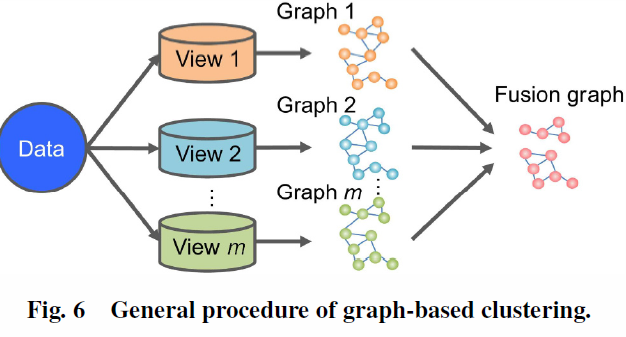
\includegraphics[width=1\textwidth]{figures/graph.png}} \label{figure_clustering}}
\caption{基于图的多视图聚类.}
\label{figure_evaluation_objective one}
}
\end{center}
\end{figure}
\end{frame}

\begin{frame}
    \frametitle{后期融合 late fusion}
    \begin{figure}[!ht]
\begin{center}
{
\centering
\subfloat[]{{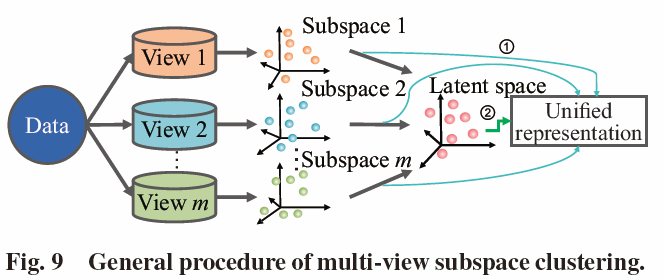
\includegraphics[width=1\textwidth]{figures/subspace.png}} \label{figure_convergence}}
\caption{基于子空间的多视图聚类}
\label{figure_evaluation_objective one}
}
\end{center}
\end{figure}
\end{frame}

\begin{frame}
    \frametitle{后期融合 late fusion}
    \begin{figure}[!ht]
\begin{center}
{
\centering
\subfloat[]{{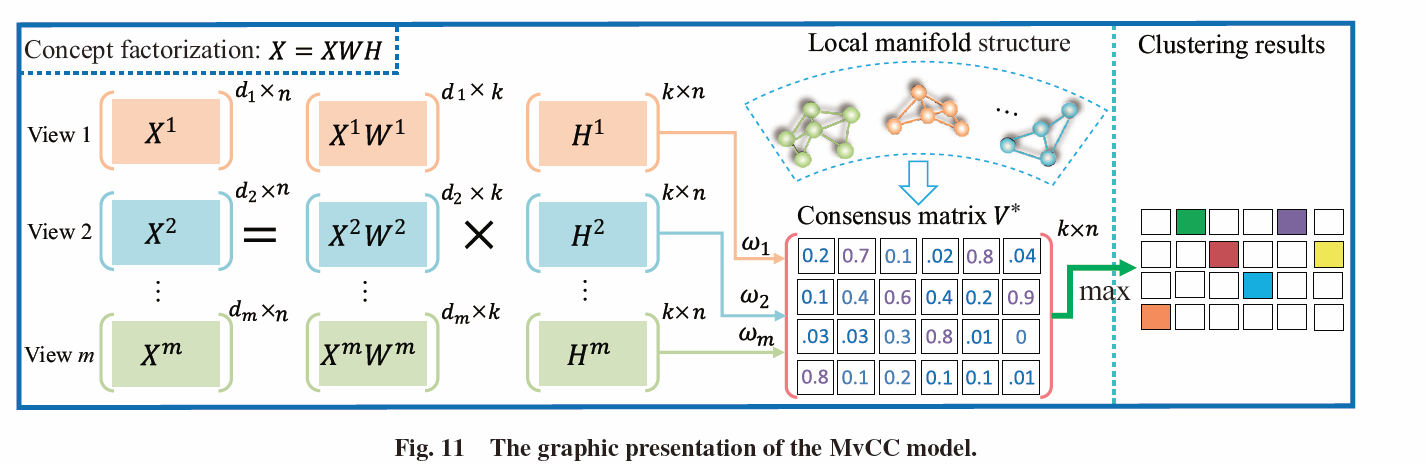
\includegraphics[width=1\textwidth]{figures/nmf.png}} \label{figure_parameter}}
\caption{基于非负矩阵分解的多视图聚类}
\label{figure_evaluation_objective one}
}
\end{center}
\end{figure}
\end{frame}

\begin{frame}
    \frametitle{后期融合 late fusion}
    \begin{figure}[!ht]
\begin{center}
{
\centering
\subfloat[]{{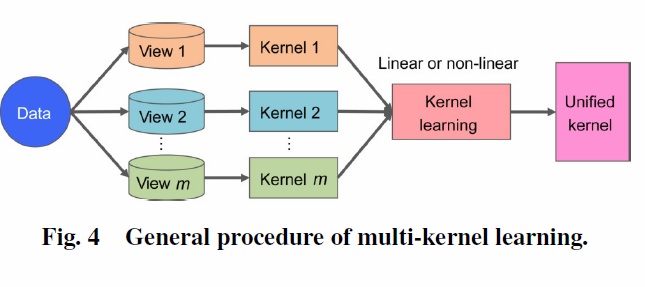
\includegraphics[width=1\textwidth]{figures/multi-kernel.png}} \label{figure_parameter}}
\caption{基于多核的多视图聚类}
}
\end{center}
\end{figure}
\end{frame}

\begin{frame}
    \frametitle{后期融合}
    \begin{itemize}
        \item 缺陷:中期融合的方法时间和空间复杂度相对都比较高,因为往往需要对相似度矩阵做SVD分解,这意味着空间复杂度为$\mathcal{O}(m n^2)$,时间复杂度为$\mathcal{O}( n^3)$;
        \item 动机:类似于ensemble learning的思想,将若干视图上取得任务结果做聚类语义上的对齐;
        \item 这里的聚类结果对应 $\{\mathbf{V}_{i}\}_{i=1}^{m}$所产生的$m$个聚类指示矩阵$\{\mathbf{H}_{i}\}_{i=1}^{m}$
        \item novelty:无监督的无标签性      
    \end{itemize}      
\end{frame}


\begin{frame}
    \frametitle{后期融合}
    \begin{itemize}
        \item 不同聚类结果之间的距离不能简单靠相减计算。
        \item 假设我们现在有5个样本和三个簇。我们从两个视图上得到了各自视图上的聚类结果如下,
\[
\mathbf{H_{1}} = \left|\begin{array}{cccc}
    1 &    0    & 0 \\
    1 &    0   & 0\\
    0 &    1   & 0 \\
    0 &    1   & 0 \\
    0 &    0   & 1
\end{array}\right|,
 \mathbf{H_{2}} = \left|\begin{array}{cccc}
    0 &    0    & 1 \\
    0 &    0   &  1\\
    1 &    0   &  0\\
    1 &    0   &  0\\
    0 &    1   &  0
\end{array}\right|
\]   
       \item 尽管数学表达形式不同,但是聚类结果一致
    \end{itemize}      
\end{frame}

\begin{frame}
    \frametitle{后期融合}
    \begin{itemize}
        \item 所以我们不能单纯地用数学意义上的范数来评估两个矩阵的相似性。对于聚类指示矩阵而言,只要能够通过列变换矩阵得到的新的聚类结果,就可以被看做与原结果等价
        \item $\mathbf{H_1} = \mathbf{H_2}\mathbf{W_2}$ 
\[
\mathbf{W_{2}} = \left|\begin{array}{cccc}
    0 &    1    & 0 \\
    0 &    0   & 1\\
    1 &    0   & 0
\end{array}\right|
\]      
    \end{itemize}      
\end{frame}

\begin{frame}
    \frametitle{后期融合}
    \begin{itemize}
        \item 优化目标
 \begin{equation}
\label{MKKM LF3}
\begin{split}
\min\limits_{\mathbf{H},\left\{\mathbf{W_p}\right\}_{p=1}^m}{\left\lVert\mathbf{H} - \frac 1m \sum_{p=1}^m \mathbf{H}_p \mathbf{W}_p\right\rVert}_{\mathbf{F}}^2,\\ ~~
s.t. ~~  \mathbf{H^{\top}}\mathbf{H} = \mathbf{I}_k, \mathbf{W^{\top}}\mathbf{W} = \mathbf{I}_k.
\end{split}
\end{equation}  

\begin{equation}
\label{MKKM LF4}
\begin{split}
\min\limits_{\mathbf{H},\left\{\mathbf{W}_p\right\}_{p=1}^m,\gamma}{\left\lVert\mathbf{H} - \sum_{p=1}^m \gamma_p \mathbf{H}_p \mathbf{W}_p\right\rVert}_{\mathbf{F}}^2,\\ ~~
s.t. ~~  \mathbf{H^{\top}}\mathbf{H} = \mathbf{I}_k, \mathbf{W^{\top}}\mathbf{W} = \mathbf{I}_k,
 \gamma^{\top}1=1,\gamma \geq 0.
\end{split}
\end{equation}   
    \end{itemize}      
\end{frame}

\begin{frame}
    \frametitle{后期融合算法}
    \begin{itemize}
        \item 后期融合通过每个视图下得到的聚类的结果,通过不同的聚类结果融合成最终的最优结果
        \item 我们是通过列变换对齐的,只要满足聚类的性质,这种对齐就可以被应用到其他领域的聚类算法上
    \end{itemize}     
      
\end{frame}

%%%%%%%%%%%%%%%%%%
\section{基于后期融合最大化的多视图聚类方法}


\begin{frame}
    \frametitle{我们的方法:MVC-LFA(Late Fusion Alignment)}
    \begin{itemize}
        \item 我们提出了基于后期融合最大化的多视图方法(ijcai-19)
    \end{itemize} 
    \begin{figure}
        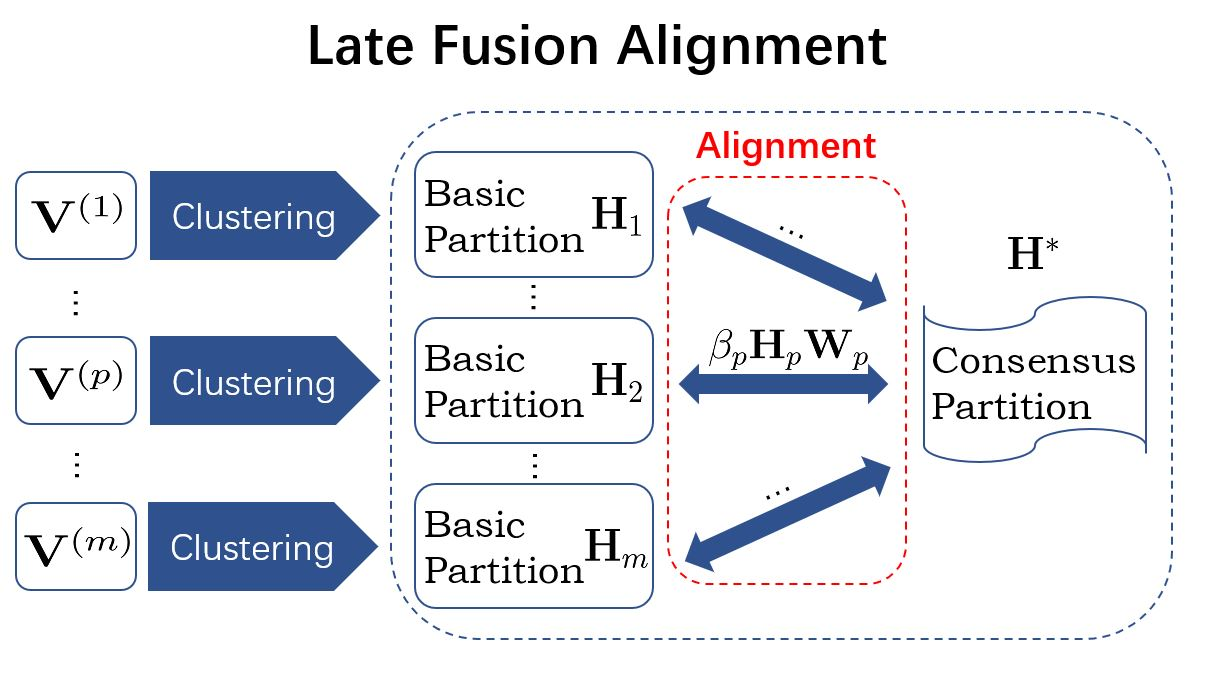
\includegraphics[width=0.9\textwidth]{figures/model3.jpg} 
    \end{figure}          
\end{frame}

\begin{frame}
    \frametitle{MVC-LFA}
    \begin{itemize}
        \item 考虑$k$-means的优化目标:
\begin{equation}\label{LFA 1}
\begin{split}
\min\nolimits_{\mathbf{H}^*}\;&\;\mathrm{Tr}(\mathbf{X} \mathbf{X}^{\mathrm{ T }}) - \mathrm{Tr} ( {\mathbf{H}^*}^{\mathrm{ T }} \mathbf{X} \mathbf{X}^{\mathrm{ T }} \mathbf{H}^*),\\
s.t. &\;  \bf{H}^* \in \mathbb{R}^{\mathit{n}\times \mathit{k}}, {\mathbf{H}^*}^{ \mathrm{ T }}\mathbf{H}^* = \mathbf{I}_k,
\end{split}
\end{equation}
         \item $\mathbf{X}$ 和 $\mathbf{H}^*$分别是数据矩阵和聚类结果矩阵。我们通过对 Eq.(\ref{LFA 1})中的$\mathbf{X} \mathbf{X}^{\mathrm{ T }}$进行SVD分解来得到最后的划分矩阵 $\mathbf{H}^*$。
         \item  当对应到多视图数据$\mathbf{X}= \sum_{p=1}^m \beta_p \mathbf{H}_p \mathbf{W}_p$时,优化过程很复杂。
    \end{itemize}   
      
\end{frame}

\begin{frame}
    \frametitle{MVC-LFA}
    \begin{itemize}
        \item 贡献一:我们首先证明了 Eq.(\ref{LFA 1})中的优化目标等价于最大化后期融合之间的对齐$\mathrm{Tr} ({\mathbf{H}^*}^{ \mathrm{ T }} \mathbf{X})$。
        \item
 \begin{proof}
因为$\mathbf{P} = {\mathbf{H}^*}^{ \mathrm{ T }} \mathbf{X}$,我们可以得到 $\mathrm{Tr}^2 ({\mathbf{H}^*}^{ \mathrm{ T }} \mathbf{X}) \leq k \cdot  \mathrm{Tr}({\mathbf{H}^*}^{ \mathrm{ T }} \mathbf{X} \mathbf{X}^{\mathrm{ T }}{\mathbf{H}^*} )$.
因此,
$
\mathrm{Tr}(\mathbf{X} \mathbf{X}^{\mathrm{ T }}) - \mathrm{Tr} ( {\mathbf{H}^*}^{\mathrm{ T }} \mathbf{X} \mathbf{X}^{\mathrm{ T }} \mathbf{H}^*) \leq 2k - \mathrm{Tr} ( {\mathbf{H}^*}^{\mathrm{ T }} \mathbf{X} \mathbf{X}^{\mathrm{ T }} \mathbf{H}^*) \leq  2k - \frac{1}{k} \mathrm{Tr}^2 ({\mathbf{H}^*}^{ \mathrm{ T }} \mathbf{X}).
$
\end{proof}
    \end{itemize} 
    
      
\end{frame}

\begin{frame}
    \frametitle{MVC-LFA优化目标}
    \begin{itemize}
        \item 根据上面的结论,我们提出了一种简单但是高效的多视图聚类算法:
        \item \begin{equation}
\label{LFA 2}
\begin{split}
\;&\;\max\nolimits_{\mathbf{H}^*,\left\{\mathbf{W}_p\right\}_{p=1}^m,\beta} \mathrm{Tr} ({\mathbf{H}^*}^{ \mathrm{ T }} \mathbf{X}) + \lambda \mathrm{Tr}({\mathbf{H}^*}^{ \mathrm{ T }} \mathbf{M}),\\
\;&\; s.t.\;{\mathbf{H}^*}^{ \mathrm{ T }}\mathbf{H}^* = \mathbf{I}_k, \mathbf{{W}}_p^{ \mathrm{ T }}\mathbf{W}_p = \mathbf{I}_k,\\
\;&\;\sum\nolimits_{p=1}^m {\beta_{p}}^2 = 1, \beta_{p} \geq 0,\mathbf{X}= \sum\nolimits_{p=1}^m \beta_p \mathbf{H}_p \mathbf{W}_p,
\end{split}
\end{equation}
    \end{itemize} 
  
      
\end{frame}

\begin{frame}
    \frametitle{MVC-LFA}
    \begin{itemize}
        \item 贡献二:我们从理论上说明了算法的收敛性:
        \item 
\begin{proof}
因为我们的优化方法采用了轮替优化法,当中每一步都是最优解,所以我们只需证明我们的算法有一个上界即可。注意到$ \forall p,q,\,\mathrm{Tr}[{(\beta_{p}\mathbf{H}_p\mathbf{W}_p)}^{\mathrm {T}} (\beta_{q}\mathbf{H}_q\mathbf{W}_q)]\leq  \mathrm{Tr}[{(\mathbf{H}_p\mathbf{W}_p)}^{\mathrm {T}} (\mathbf{H}_q\mathbf{W}_q)] \leq \frac{1}{2} (\mathrm{Tr} [{(\mathbf{H}_p\mathbf{W}_p)}^{\mathrm {T}} {(\mathbf{H}_p\mathbf{W}_p)}]  + \mathrm{Tr} [{(\mathbf{H}_q\mathbf{W}_q)}^{\mathrm {T}} {(\mathbf{H}_q\mathbf{W}_q)}]) = k$. $\mathrm{Tr} ({\mathbf{H}^*}^{ \mathrm{ T }} \mathbf{X})  \leq \frac{1}{2} (\mathrm{Tr} [{\mathbf{H}^*}^{\mathrm {T}} {\mathbf{H}^*}]  + \mathrm{Tr} [{\mathbf{X}}^{\mathrm {T}} {\mathbf{X}}]) \!= \! \frac{1}{2} (\mathrm{Tr} [{\mathbf{H}^*}^{\mathrm {T}} {\mathbf{H}^*}]  + \mathrm{Tr} (\sum_{p,q=1}^m {(\beta_{p}\mathbf{H}_p\mathbf{W}_p)}^{\mathrm {T}} (\beta_{q}\mathbf{H}_q\mathbf{W}_q))) \leq \frac{k}{2} (m^2+1)$. 同时, the $({\mathbf{H}^*}^{ \mathrm{ T }} \mathbf{M}) \leq  \frac{1}{2} (\mathrm{Tr} [{\mathbf{H}^*}^{\mathrm {T}} {\mathbf{H}^*}]  + \mathrm{Tr} [{\mathbf{M}}^{\mathrm {T}} {\mathbf{M}}]) = k$. 
\end{proof}

    \end{itemize} 
 
      
\end{frame}

\begin{frame}
    \frametitle{MVC-LFA}
    \begin{itemize}
        \item 实验数据 
\begin{table}[!t]
\begin{center}
{
\caption{{Datasets used in our experiments.}}\label{dataset table}
\begin{tabular}{c||c|c|c}
\toprule
Dataset         & \#Samples   & \#Views & \#Classes\\
\midrule
Flower17        &  $1360$    & $7$           & $17$\\
\hline
ProteinFold     &  $694$     & $12$          & $27$\\
\hline
Flower102       &  $8189$    & $4$           & $102$\\
\hline
Caltech         &  $1530$    & $25$          & $102$\\
\hline
CCV             &  $6773$    & $3$           & $20$\\
\bottomrule
\end{tabular}
}
\end{center}
\vspace{-15pt}
\end{table}
    \end{itemize} 
  
      
\end{frame}

\begin{frame}
    \frametitle{MVC-LFA}
    \begin{itemize}
        \item 实验结果
\begin{table}[!htbp]
\begin{center}
{
  \centering
  \caption{{ACC, NMI and purity comparison of different clustering algorithms on five benchmark data sets.}}\label{results table}
  \resizebox{\textwidth}{!}{
    \begin{tabular}{|c|c|c|c|c|c|c|c|c|c|}
    \toprule
    \multirow{2}{*}{Datasets}      & \multirow{2}{*}{{A-MKKM}}   & \multirow{2}{*}{{SB-KKM}} & {{MKKM}} & {OKKC} & {CSRC} & MKC-LKA & MKKM-MR &ONKC &  \multirow{2}{*}{Proposed} \\
     &    & & \small{\cite{huang2012multiple}} & \small \cite{Yu2012Optimized} & \small{\cite{kumar2011co}} & \small \cite{Li2016Multiple} & \small \cite{Liu2016Multiple} &  \small{\cite{liu2017optimal}} & \\
    \midrule
    \multicolumn{10}{|c|} {ACC$(\%)$} \\
    \hline
    Flower17 & 51.03  & 42.06  & 45.37 &44.85   & 51.76  &60.69  & 59.69   & 60.88 & \textbf{\color{red}62.16}  \\
    \hline
    ProteinFold & 30.69  & 34.58  & 27.23 &37.10 & 35.59  & 39.34  & 36.89    & 37.90     & \textbf{\color{red}41.49}  \\
    \hline
    Flower102 & 27.29  & 33.13  & 21.96  &22.32  & 38.60  & 40.84  & 40.24     & 37.32        & \textbf{\color{red}44.16}    \\
    \hline
    Caltech & 35.56  & 33.14  & 34.77  &33.92 & 34.38  & 36.06  & 35.82   & 35.32  & \textbf{\color{red}38.39}  \\
    \hline
    CCV     & 19.74  &20.08   &18.01   &20.54  &23.06   &23.49  &22.47    & 24.18 &  \textbf{\color{red} 27.56}       \\
    \midrule
    \multicolumn{10}{|c|}{NMI$(\%)$} \\
    \hline
    Flower17 & 50.19  & 45.14  & 45.35  &45.85 & 53.19  & 57.27  & 57.11   & 58.58 &  \textbf{\color{red}60.79}  \\
    \hline
    ProteinFold & 40.96  & 42.33  & 37.16  &40.75  & 45.66  & 47.55  & 45.13  & 46.93     &\textbf{\color{red}49.96}  \\
    \hline
    Flower102 & 46.32  & 48.99  & 42.30  &43.28 & 54.95  & 57.60  & 57.27   & 58.13      & \textbf{\color{red}60.48}  \\
    \hline
    Caltech & 59.90  & 59.07  & 59.64  &57.22 & 58.35  & 60.98  & 60.18   & 60.41 & \textbf{\color{red}62.65}      \\
    \hline
    CCV     &17.16    &17.73   &15.52  &16.28 &18.89   &17.11   &18.62     & 18.24  &\textbf{\color{red} 20.59}   \\
    \midrule
    \multicolumn{10}{|c|}{Purity$(\%)$} \\
    \hline
    Flower17 & 51.99  & 44.63  & 46.84 &45.00 & 53.68  & 61.79  & 60.03  &  61.64 &  \textbf{\color{red}63.32}       \\
    \hline
    ProteinFold & 37.18  & 41.21  & 33.86 &39.91 & 42.07  & 45.97  & 43.80   & 45.24     &  \textbf{\color{red}48.85}  \\
    \hline
    Flower102 & 32.28  & 38.74  & 27.61 &28.12 & 45.04  & 48.21  & 46.39     & 47.64     &  \textbf{\color{red}50.44} \\
    \hline
    Caltech & 37.12  & 35.10  & 37.25  &36.27 & 35.95  & 38.08  & 37.65     & 39.08 & \textbf{\color{red}41.28}     \\
    \hline
    CCV     & 23.98  &23.48   &22.25  &24.17  &26.80   &22.93  &25.69      & 23.34  & \textbf{\color{red}30.71}    \\
    \bottomrule
    \end{tabular}}
    }
\end{center}
\end{table}
    \end{itemize}   
      
\end{frame}

\begin{frame}
    \frametitle{我们的方法:MVC-LFA(Late Fusion Alignment)}
    \begin{itemize}
        \item 实验结果验证了我们所提出的优化目标的有效性
\begin{figure}[!ht]
\vspace{-15pt}
\begin{center}
{
\centering
\subfloat[]{{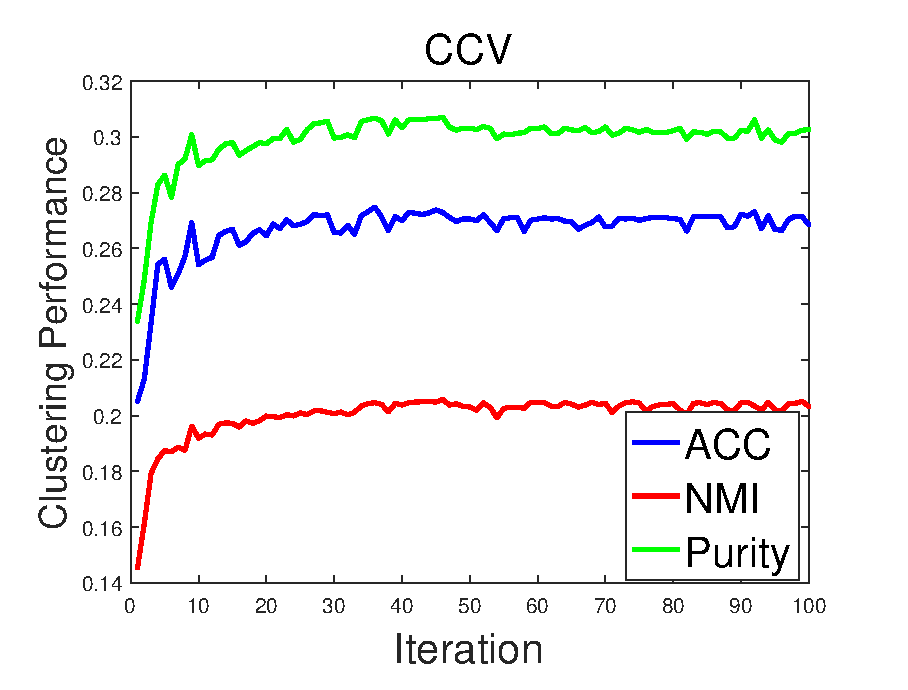
\includegraphics[width=0.5\textwidth]{figures/clusteringpictures.eps}} \label{figure_clustering}}%
\subfloat[]{{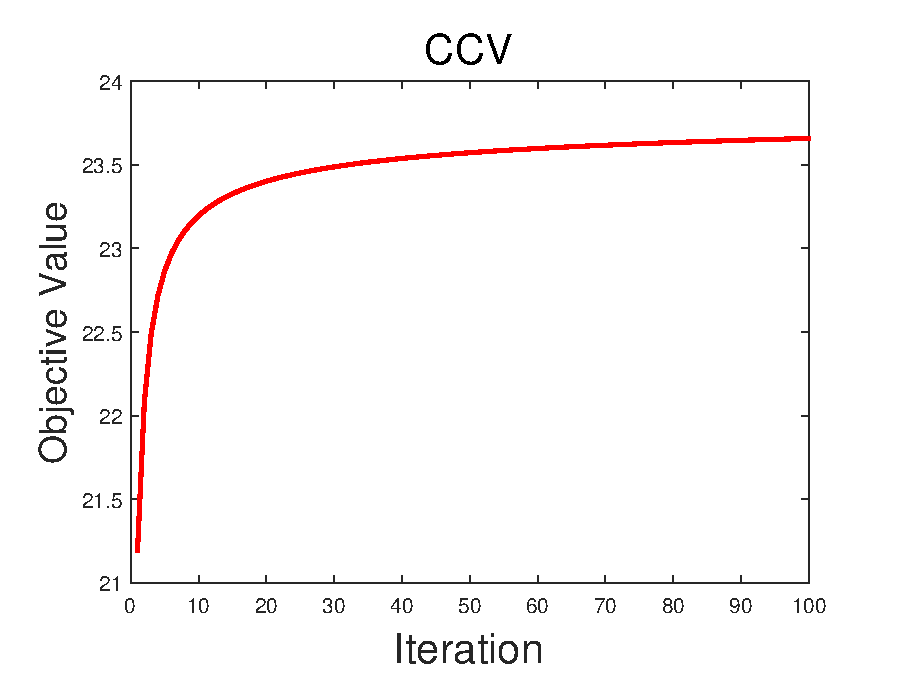
\includegraphics[width=0.5\textwidth]{figures/convergence.eps}} \label{figure_convergence}}%
\vspace{-11pt}
\caption{}
}
\end{center}
\end{figure}
    \end{itemize} 
        
\end{frame}

\begin{frame}
    \frametitle{我们的方法:MVC-LFA(Late Fusion Alignment)}
    \begin{itemize}
        \item 时间上从$\mathcal{O}(n^3)$降到了$\mathcal{O}(n)$
    \end{itemize} 
    \begin{figure}
        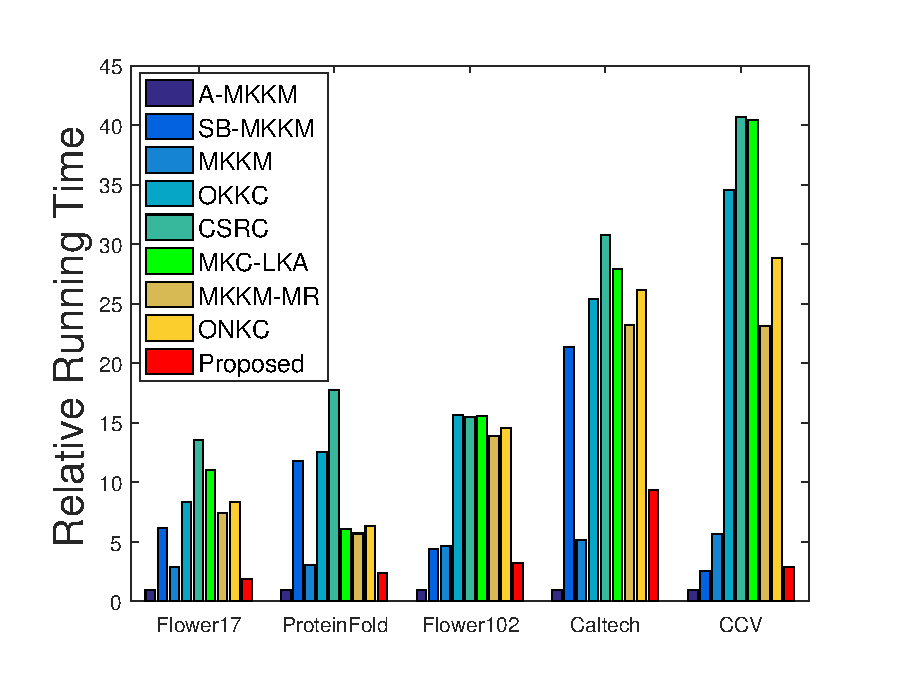
\includegraphics[width=0.8\textwidth]{figures/timepictures.eps} 
    \end{figure}          
\end{frame}

%%%%%%%%%%%%%%%%%%%
\section{无人机竞赛}

\begin{frame}
    \frametitle{无人机目标检测竞赛}
    \begin{itemize}
        \item 在已有的无人机云台上,需要我们去建立算法来实现目标检测
        \item one-stage和two-stage的目标检测算法的迁移
        \item 空军的迫切需求
        \item 学术转到工程上的考虑:实际需求
    \end{itemize}
\end{frame}

\begin{frame}
    \frametitle{缺失k-means聚类}
    \begin{itemize}
        \item 首届空军主办的无人机挑战赛,在西安举办
    \end{itemize} 
    \begin{figure}
        \includegraphics[width=0.9\textwidth]{12.jpg} 
    \end{figure}          
\end{frame}

\begin{frame}
    \frametitle{无人机目标检测竞赛}
    \begin{itemize}
        \item 现有的识别方法基于传统的CV算法,如hough圆变换等等,但是会有很多不确定因素
        \item 比如目标是红色,但是不同的天气下红色在图像中的像素不一样,会导致错检甚至于无法识别
        \item 深度学习的方法是可以来处理这些变化的,基于纹理特征
        \item 此次采用的是retinanet来处理
    \end{itemize}
\end{frame}

\begin{frame}
    \frametitle{无人机目标检测竞赛}
    \begin{itemize}
        \item 首届空军主办的无人机挑战赛,在西安举办
    \end{itemize} 
    \begin{figure}
        \includegraphics[width=0.9\textwidth]{13.jpg} 
    \end{figure}          
\end{frame}

\begin{frame}
    \frametitle{无人机目标检测竞赛}
    \begin{itemize}
        \item 首届空军主办的无人机挑战赛,在西安举办
    \end{itemize} 
    \begin{figure}
        \includegraphics[width=0.4\textwidth]{14.jpg} 
    \end{figure}          
\end{frame}

\begin{frame}
    \frametitle{比赛不足}
    \begin{itemize}
        \item 训练不够充分,设备未准备好
        \item 图传性能不好,传回的图片质量较差
        \item 无人机的高度不固定的时候,目标的尺度不一,而此次比赛就缺少对于小样本的注意力
        \item 机载和工作站的区别
    \end{itemize}
\end{frame}
%%\subsection{域适配问题 (domain adaptation)}
\begin{frame}
    \frametitle{迁移学习:域适配问题}
    \begin{itemize}
        \item 域适配问题
            \begin{itemize}
                \item domain adaptation, cross-domain learning
                \item 问题定义:有标签的源域和无标签的目标域共享相同的特征和类别,但是特征分布不同,如何利用源域标定目标域.
                $\mathcal{D}_S \neq \mathcal{D}_T: P_S(X) \neq P_T(X)$
            \end{itemize}
    \end{itemize}
    \begin{figure}
        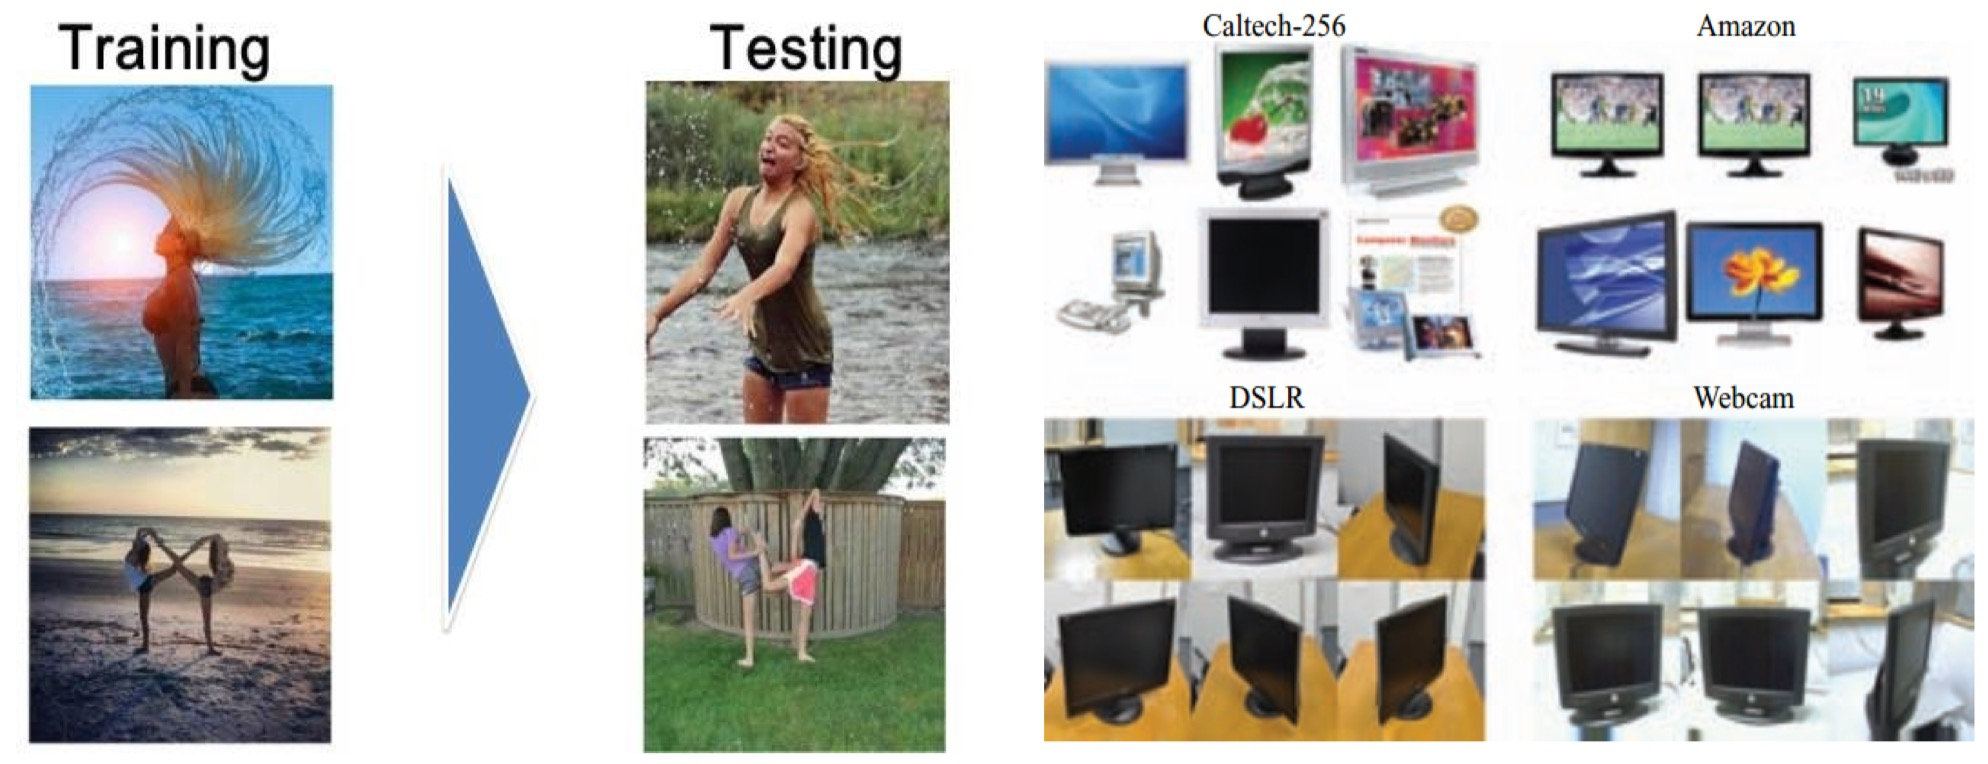
\includegraphics[width=0.9\textwidth]{da.jpg}
    \end{figure}
\end{frame}

\begin{frame}
    \frametitle{迁移学习:域适配问题}
    \begin{itemize}
        \item 域适配问题
            \begin{itemize}
                \item 基于特征的迁移方法:
                    \begin{itemize}
                        \item Transfer component analysis [Pan, TKDE-11]
                        \item Geodesic flow kernel [Duan, CVPR-12]
                        \item Transfer kernel learning [Long, TKDE-15]
                        \item TransEMDT [Zhao, IJCAI-11]
                    \end{itemize}
                \item 基于实例的迁移方法:
                    \begin{itemize}
                        \item Kernel mean matching [Huang, NIPS-06]
                        \item Covariate Shift Adaptation [Sugiyama, JMLR-07]
                    \end{itemize}
                \item 基于模型的迁移方法:
                    \begin{itemize}
                        \item Adaptive SVM (ASVM) [Yang et al, ACM Multimedia-07]
                        \item Multiple Convex Combination (MCC) [Schweikert, NIPS-09]
                        \item Domain Adaptation Machine (DAM) [Duan, TNNLS-12]
                    \end{itemize}
            \end{itemize}
    \end{itemize}
\end{frame}

\begin{frame}
    \frametitle{迁移学习:域适配问题}
    \begin{itemize}
        \item 迁移成分分析 (TCA, transfer component analysis) \footfullcite{ijcai2009-200}
            \begin{itemize}
                \item 将源域和目标域变换到相同空间,最小化它们的距离
            \end{itemize}
    \end{itemize}
    \begin{figure}
        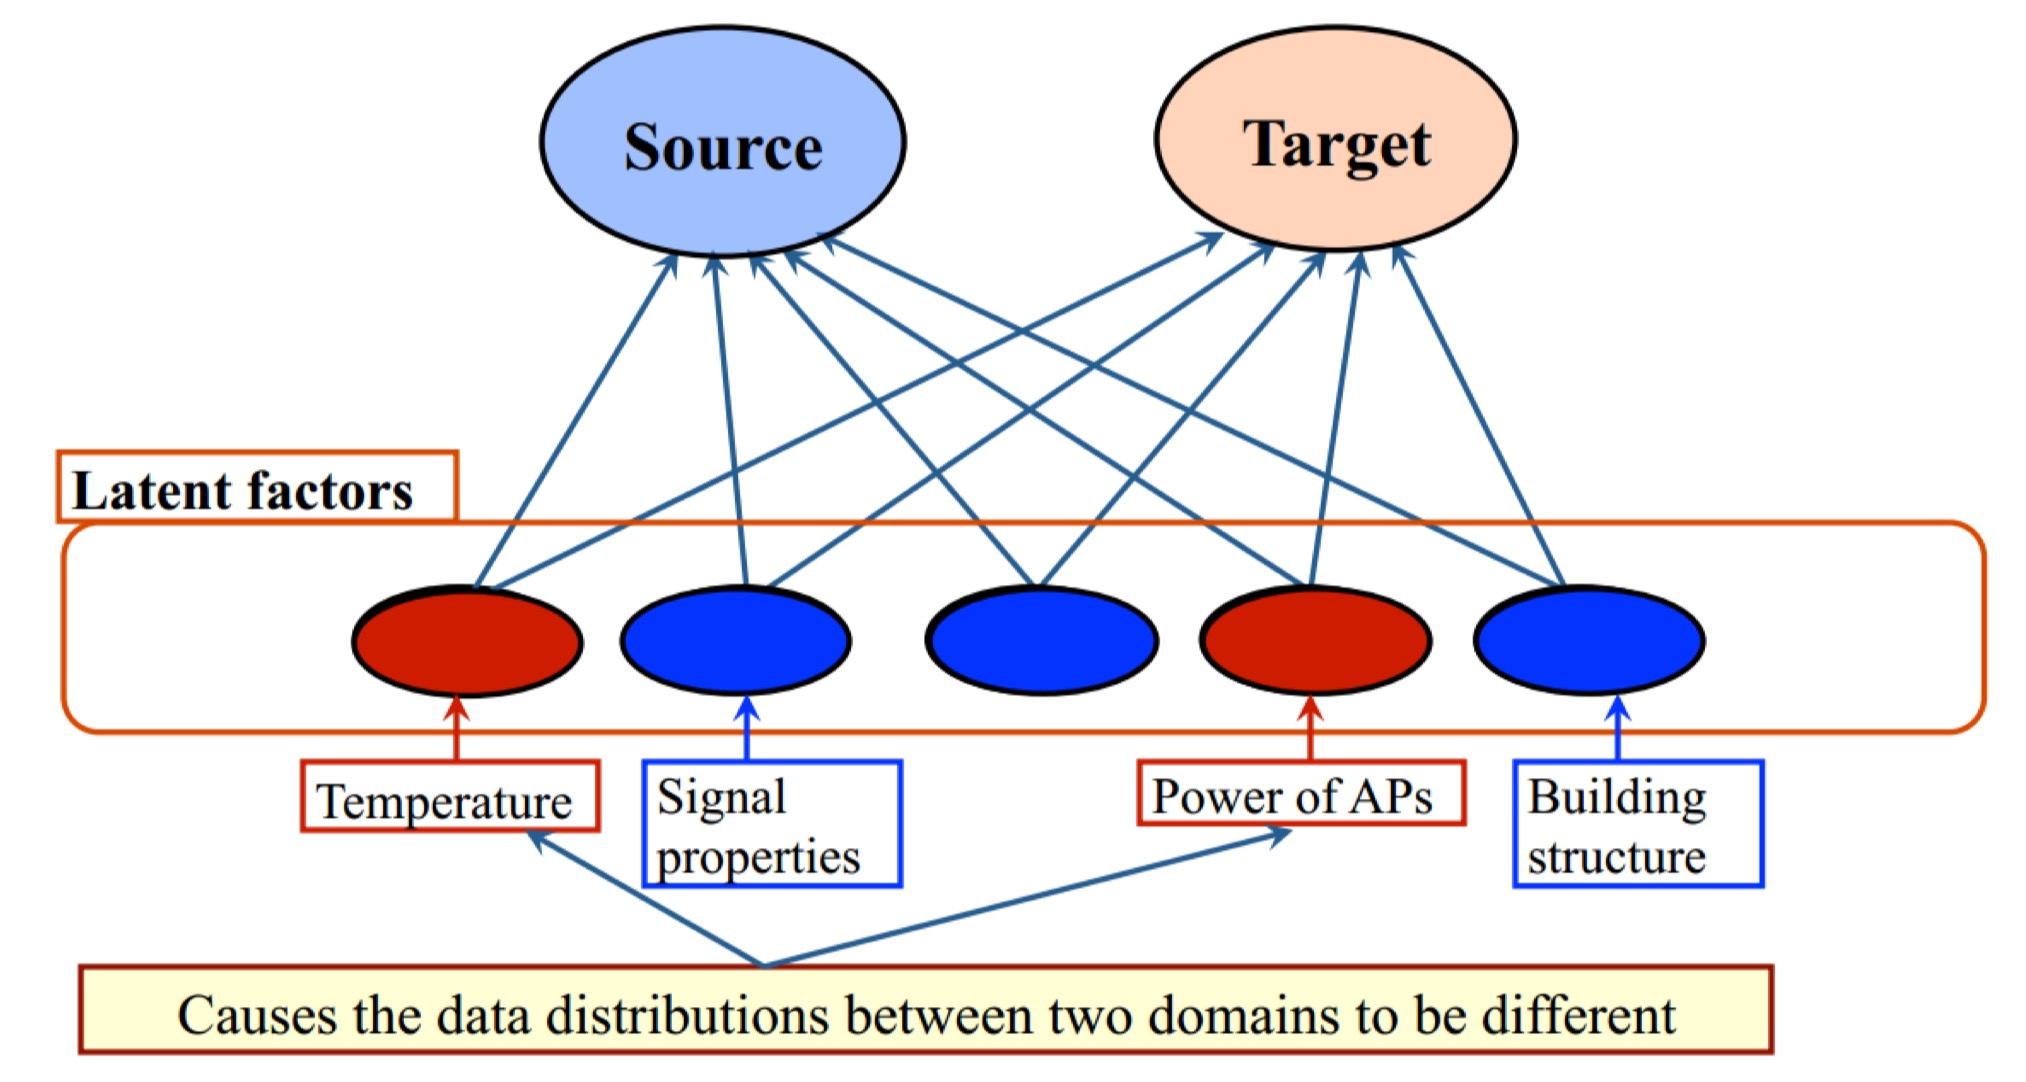
\includegraphics[width=0.9\textwidth]{tca.jpg}
    \end{figure}
\end{frame}

\begin{frame}
    \frametitle{迁移学习:域适配问题}
    \begin{itemize}
        \item 迁移成分分析 (TCA, transfer component analysis)
            \begin{itemize}
                \item 优化目标 (s.t. constraints on $\varphi(X_S)$, $\varphi(X_T)$)
                $$\max_{\varphi}\  \text{Dist}(\varphi(X_S),\varphi(X_T)) + \lambda \Omega(\varphi)$$
                \item Maximum mean discrepancy (MMD)
                $$\text{Dist}[P(X_S),P(X_T)] \triangleq\Vert \frac{1}{n_S}\sum\limits_{i=1}^{n_S}\phi(x_{S_i})-\frac{1}{n_T}\sum\limits_{j=1}^{n_T}\phi(x_{T_j})\Vert_{\mathcal{H}}$$
            \end{itemize}
    \end{itemize}
    \begin{figure}
        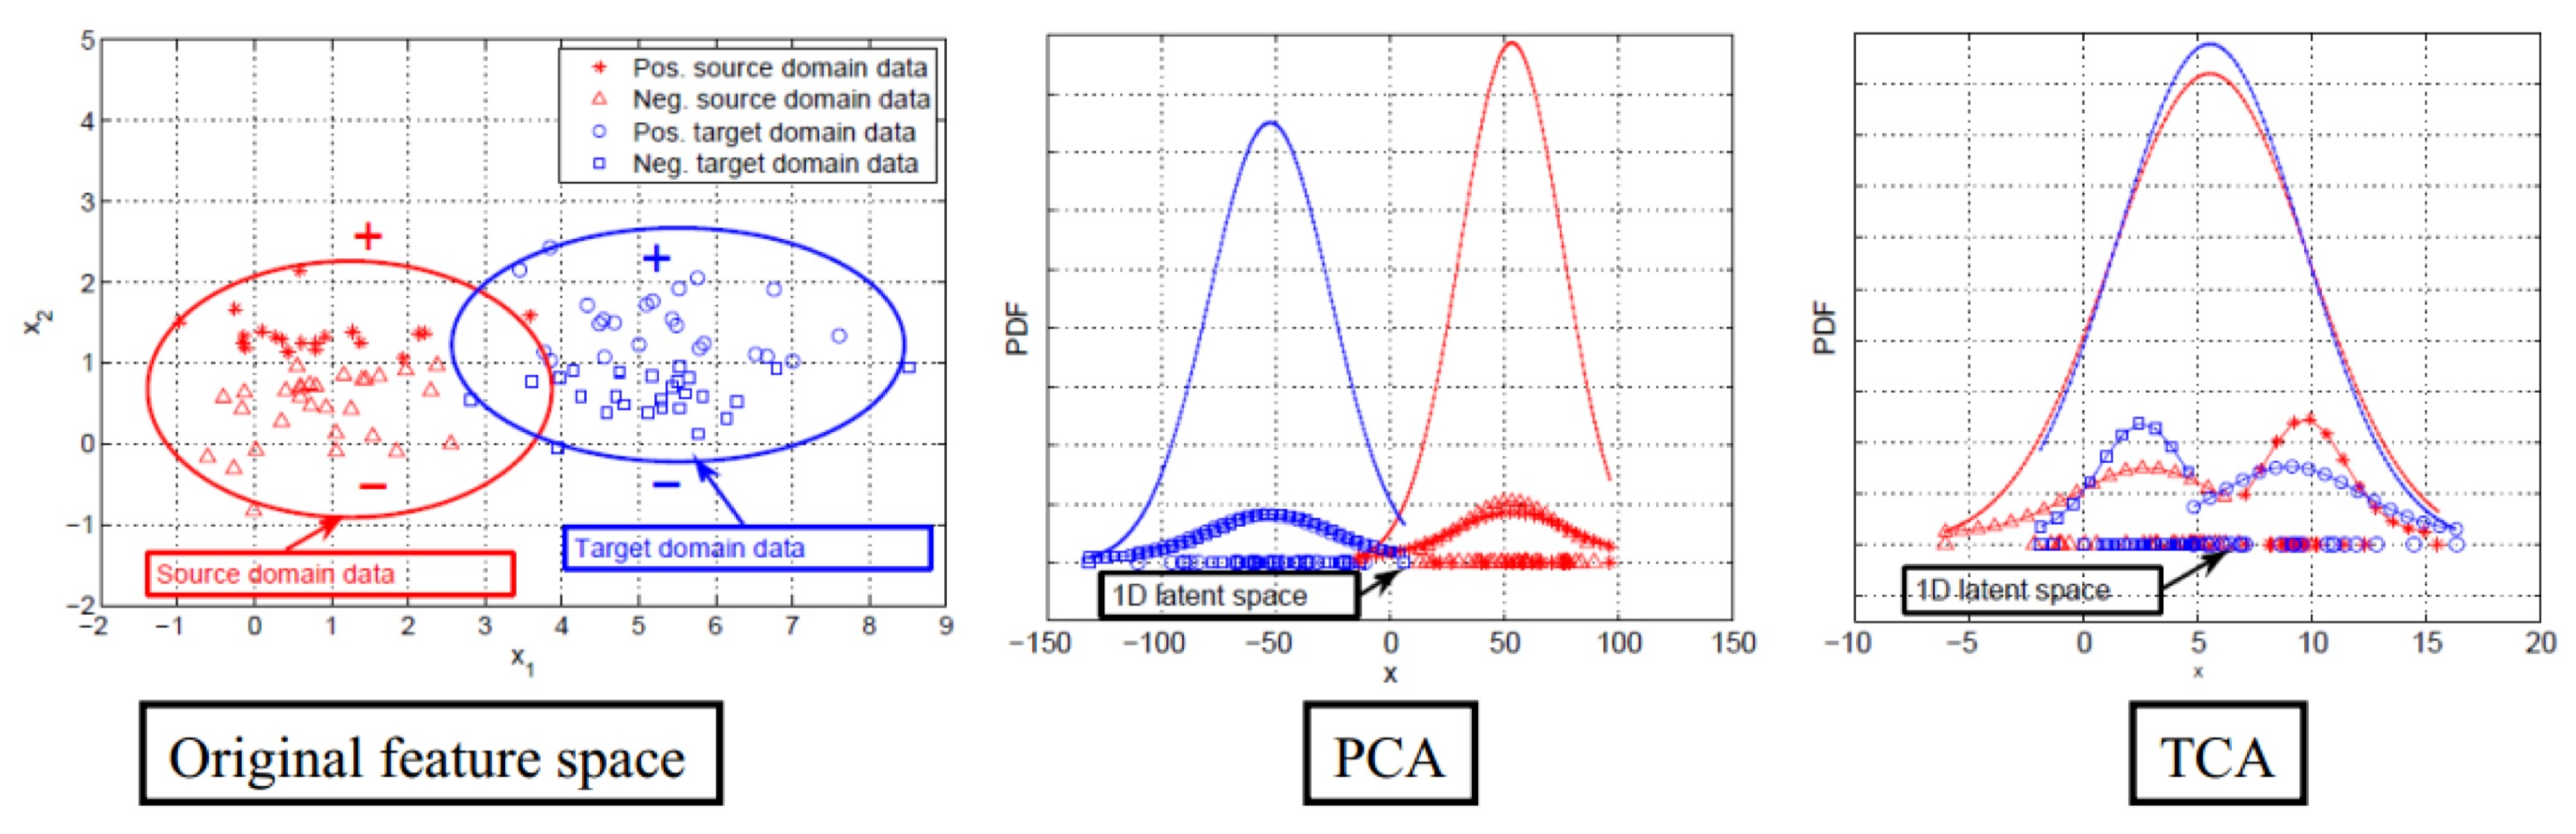
\includegraphics[width=0.8\textwidth]{tca2.jpg}
    \end{figure}
\end{frame}

\begin{frame}
    \frametitle{迁移学习:域适配问题}
    \begin{itemize}
        \item GFK (geodesic flow kernel) \footfullcite{gong2012geodesic}
            \begin{itemize}
                \item 利用流形学习,将数据映射到高维空间中,然后测量其距离 ,使得源域和目标域差异最大
                \item 优化目标
                    $$\Phi(t)=P_S U_1\Gamma(t) - R_S U_2\Sigma(t)$$
                    $$P_S^T P_{\mathcal{T}} = U_1 \Gamma V^T, R_S^T P_{\mathcal{T}} = -U_2 \Sigma V^T$$
                \item 流形正则项
                $\mathcal{R(S,T)} = \frac{1}{d^*} \sum_i^{d^*} \theta_i[\text{KL}(\mathcal{S}_i\parallel \mathcal{T}_i) + \text{KL}(\mathcal{T}_i\parallel \mathcal{S}_i)]
                $
            \end{itemize}
    \end{itemize}
    \begin{figure}
        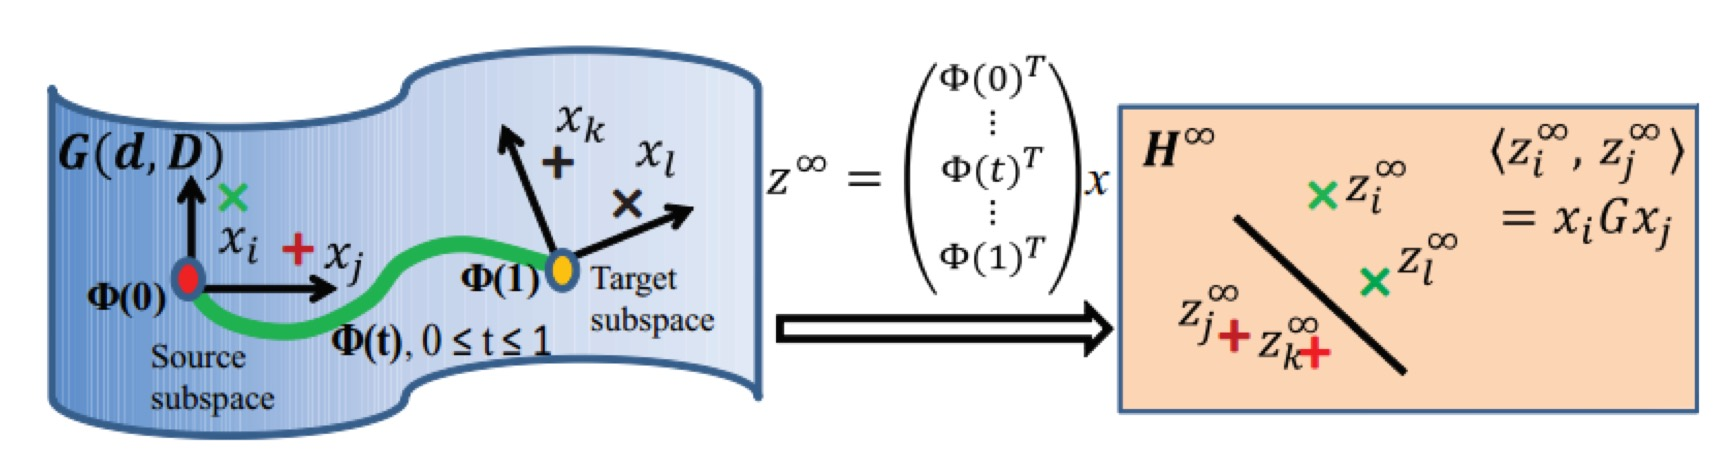
\includegraphics[width=0.7\textwidth]{gfk.jpg}
    \end{figure}
\end{frame}

\begin{frame}
    \frametitle{迁移学习:域适配问题}
    \begin{itemize}
        \item Transfer Kernel Learning (TKL) \footfullcite{long2015domain}
            \begin{itemize}
                \item 在再生核希尔伯特空间中学习一个领域不变核矩阵,从而实现源域和目标域的适配
                \item 优化目标
                $$\min_{\Lambda} \lVert \bar{\mathbf{K}}_{\mathcal Z} - \mathbf{K}_{\mathcal Z} \rVert^2_F = \lVert \bar{\Phi}_{\mathcal{Z}} \Lambda
\bar{\Phi}_{\mathcal{Z}}^{\text{T}}- \mathbf{K}_{\mathcal Z} \rVert ^2_F $$
                $$\lambda_i \geq \zeta\lambda_{i+1}, i=1,...,n-1$$
                $$\lambda_i \geq 0, i=1,...,n$$
            \end{itemize}
    \end{itemize}
    \begin{figure}
        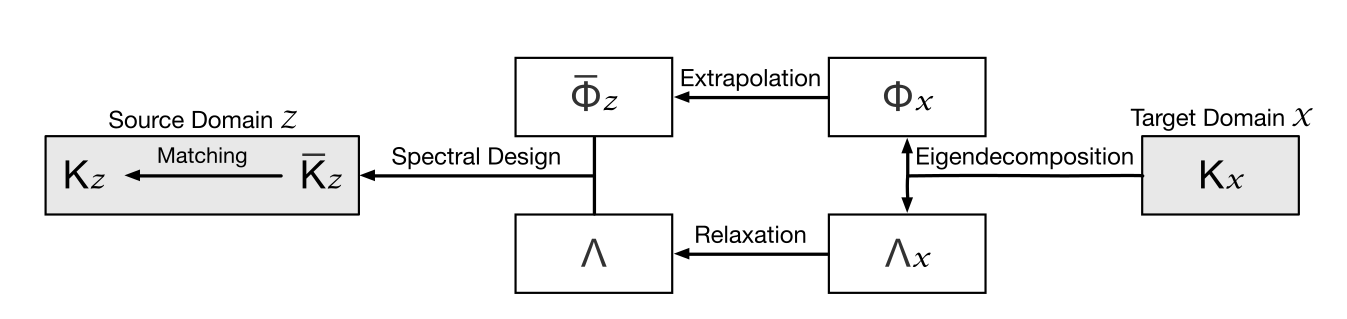
\includegraphics[width=0.9\textwidth]{tkl.png}
    \end{figure}
\end{frame}

\begin{frame}
    \frametitle{迁移学习:域适配问题}
    \begin{itemize}
        \item 嵌入决策树算法 (TransEMDT) \footfullcite{zhao2011cross}
            \begin{itemize}
                \item 首先通过聚类得到初始的目标域决策树模型,然后迭代更新决策树的参数直到收敛为止
            \end{itemize}
    \end{itemize}
    \begin{figure}
        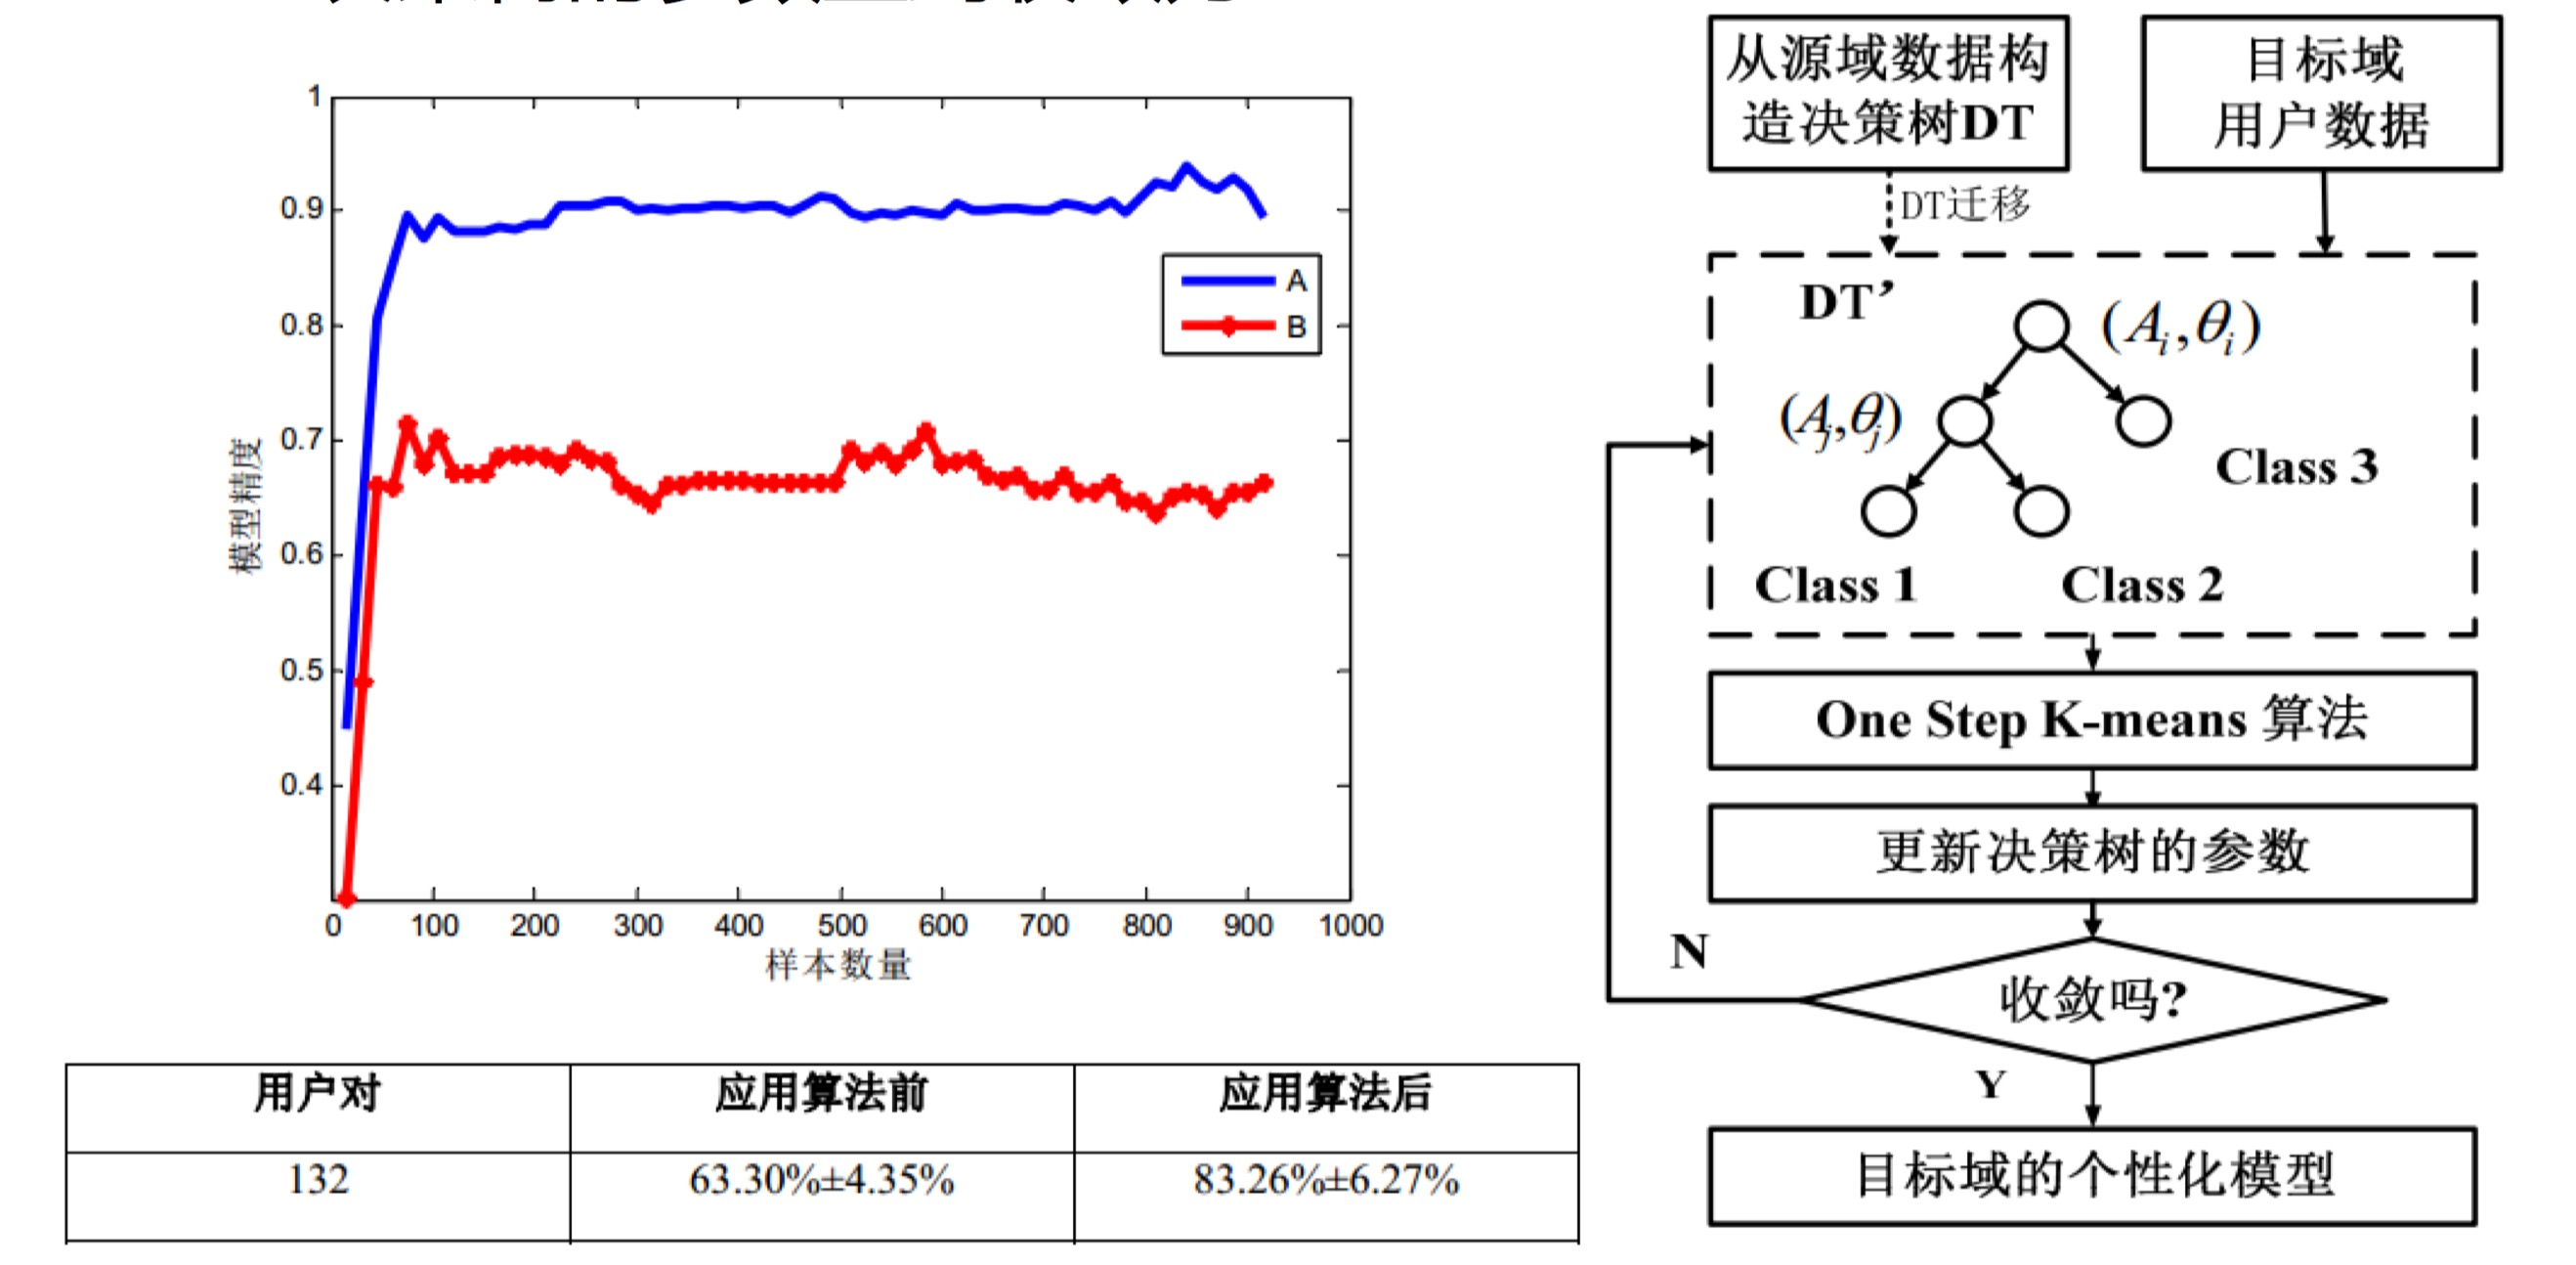
\includegraphics[width=0.9\textwidth]{tremdt.jpg}
    \end{figure}
\end{frame}

\begin{frame}
    \frametitle{迁移学习:域适配问题}
    \begin{itemize}
        \item Kernel mean matching \footfullcite{huang2007correcting}
            \begin{itemize}
                \item 在再生希尔伯特空间中计算源域和目标域的协方差分布差异 ,然后用二次规划求解样本权重
                \item 优化目标
            \end{itemize}
    \end{itemize}
    \begin{figure}
        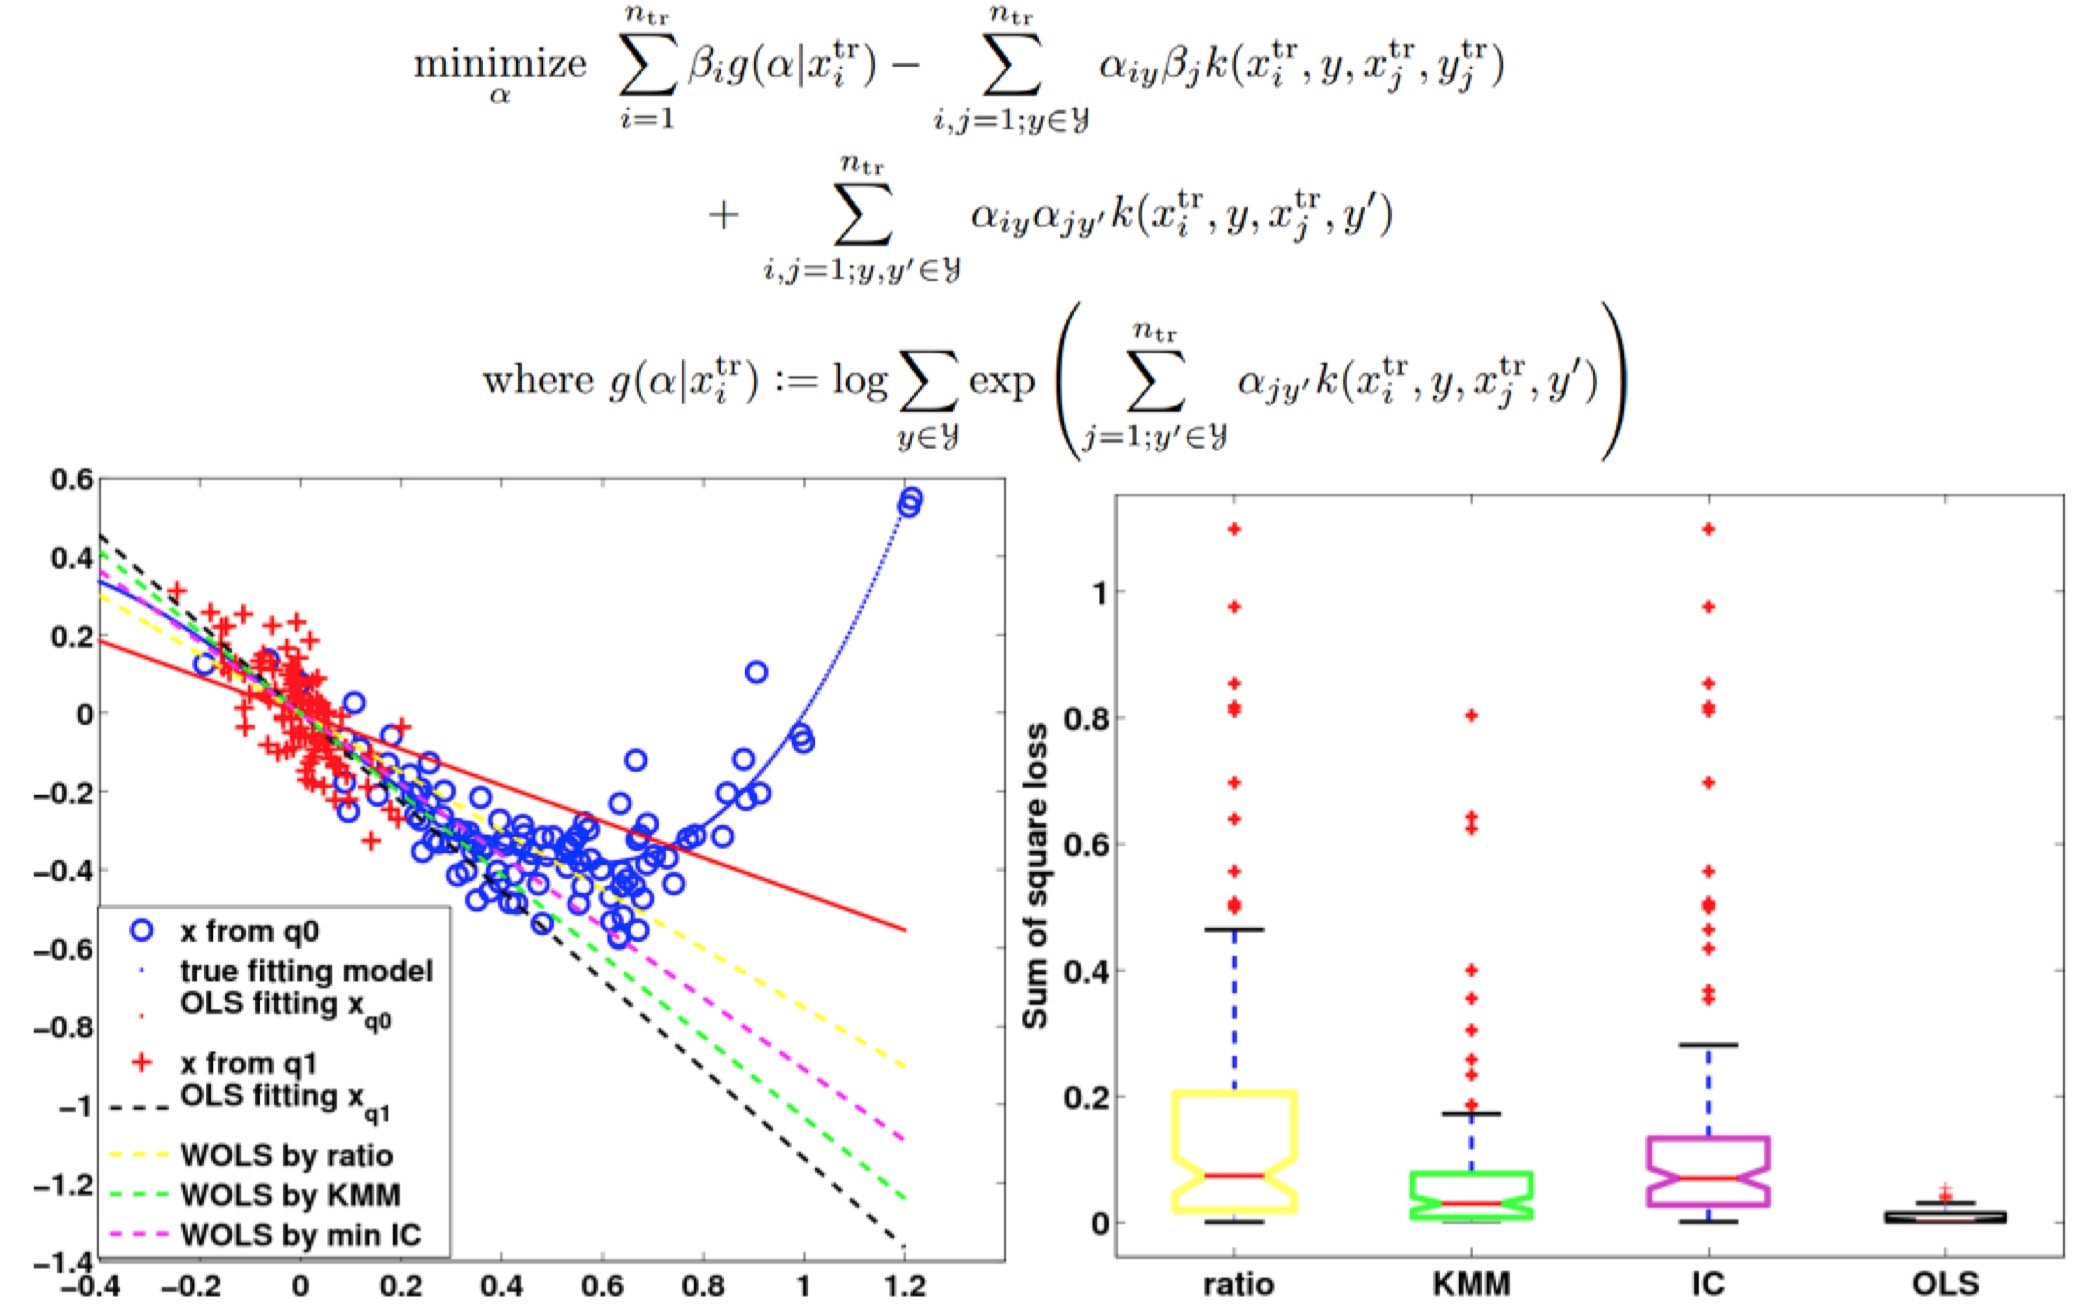
\includegraphics[width=0.6\textwidth]{kmm.jpg}
    \end{figure}
\end{frame}

\begin{frame}
    \frametitle{迁移学习:域适配问题}
    \begin{itemize}
        \item Covariate Shift Adaptation \footfullcite{wu2013learning}
            \begin{itemize}
                \item 采用自然估计法估计源域和目标域的密度比例,然后进行实 例权重的分配,最后迁移
                \item 优化目标
            \end{itemize}
    \end{itemize}
    \begin{figure}
        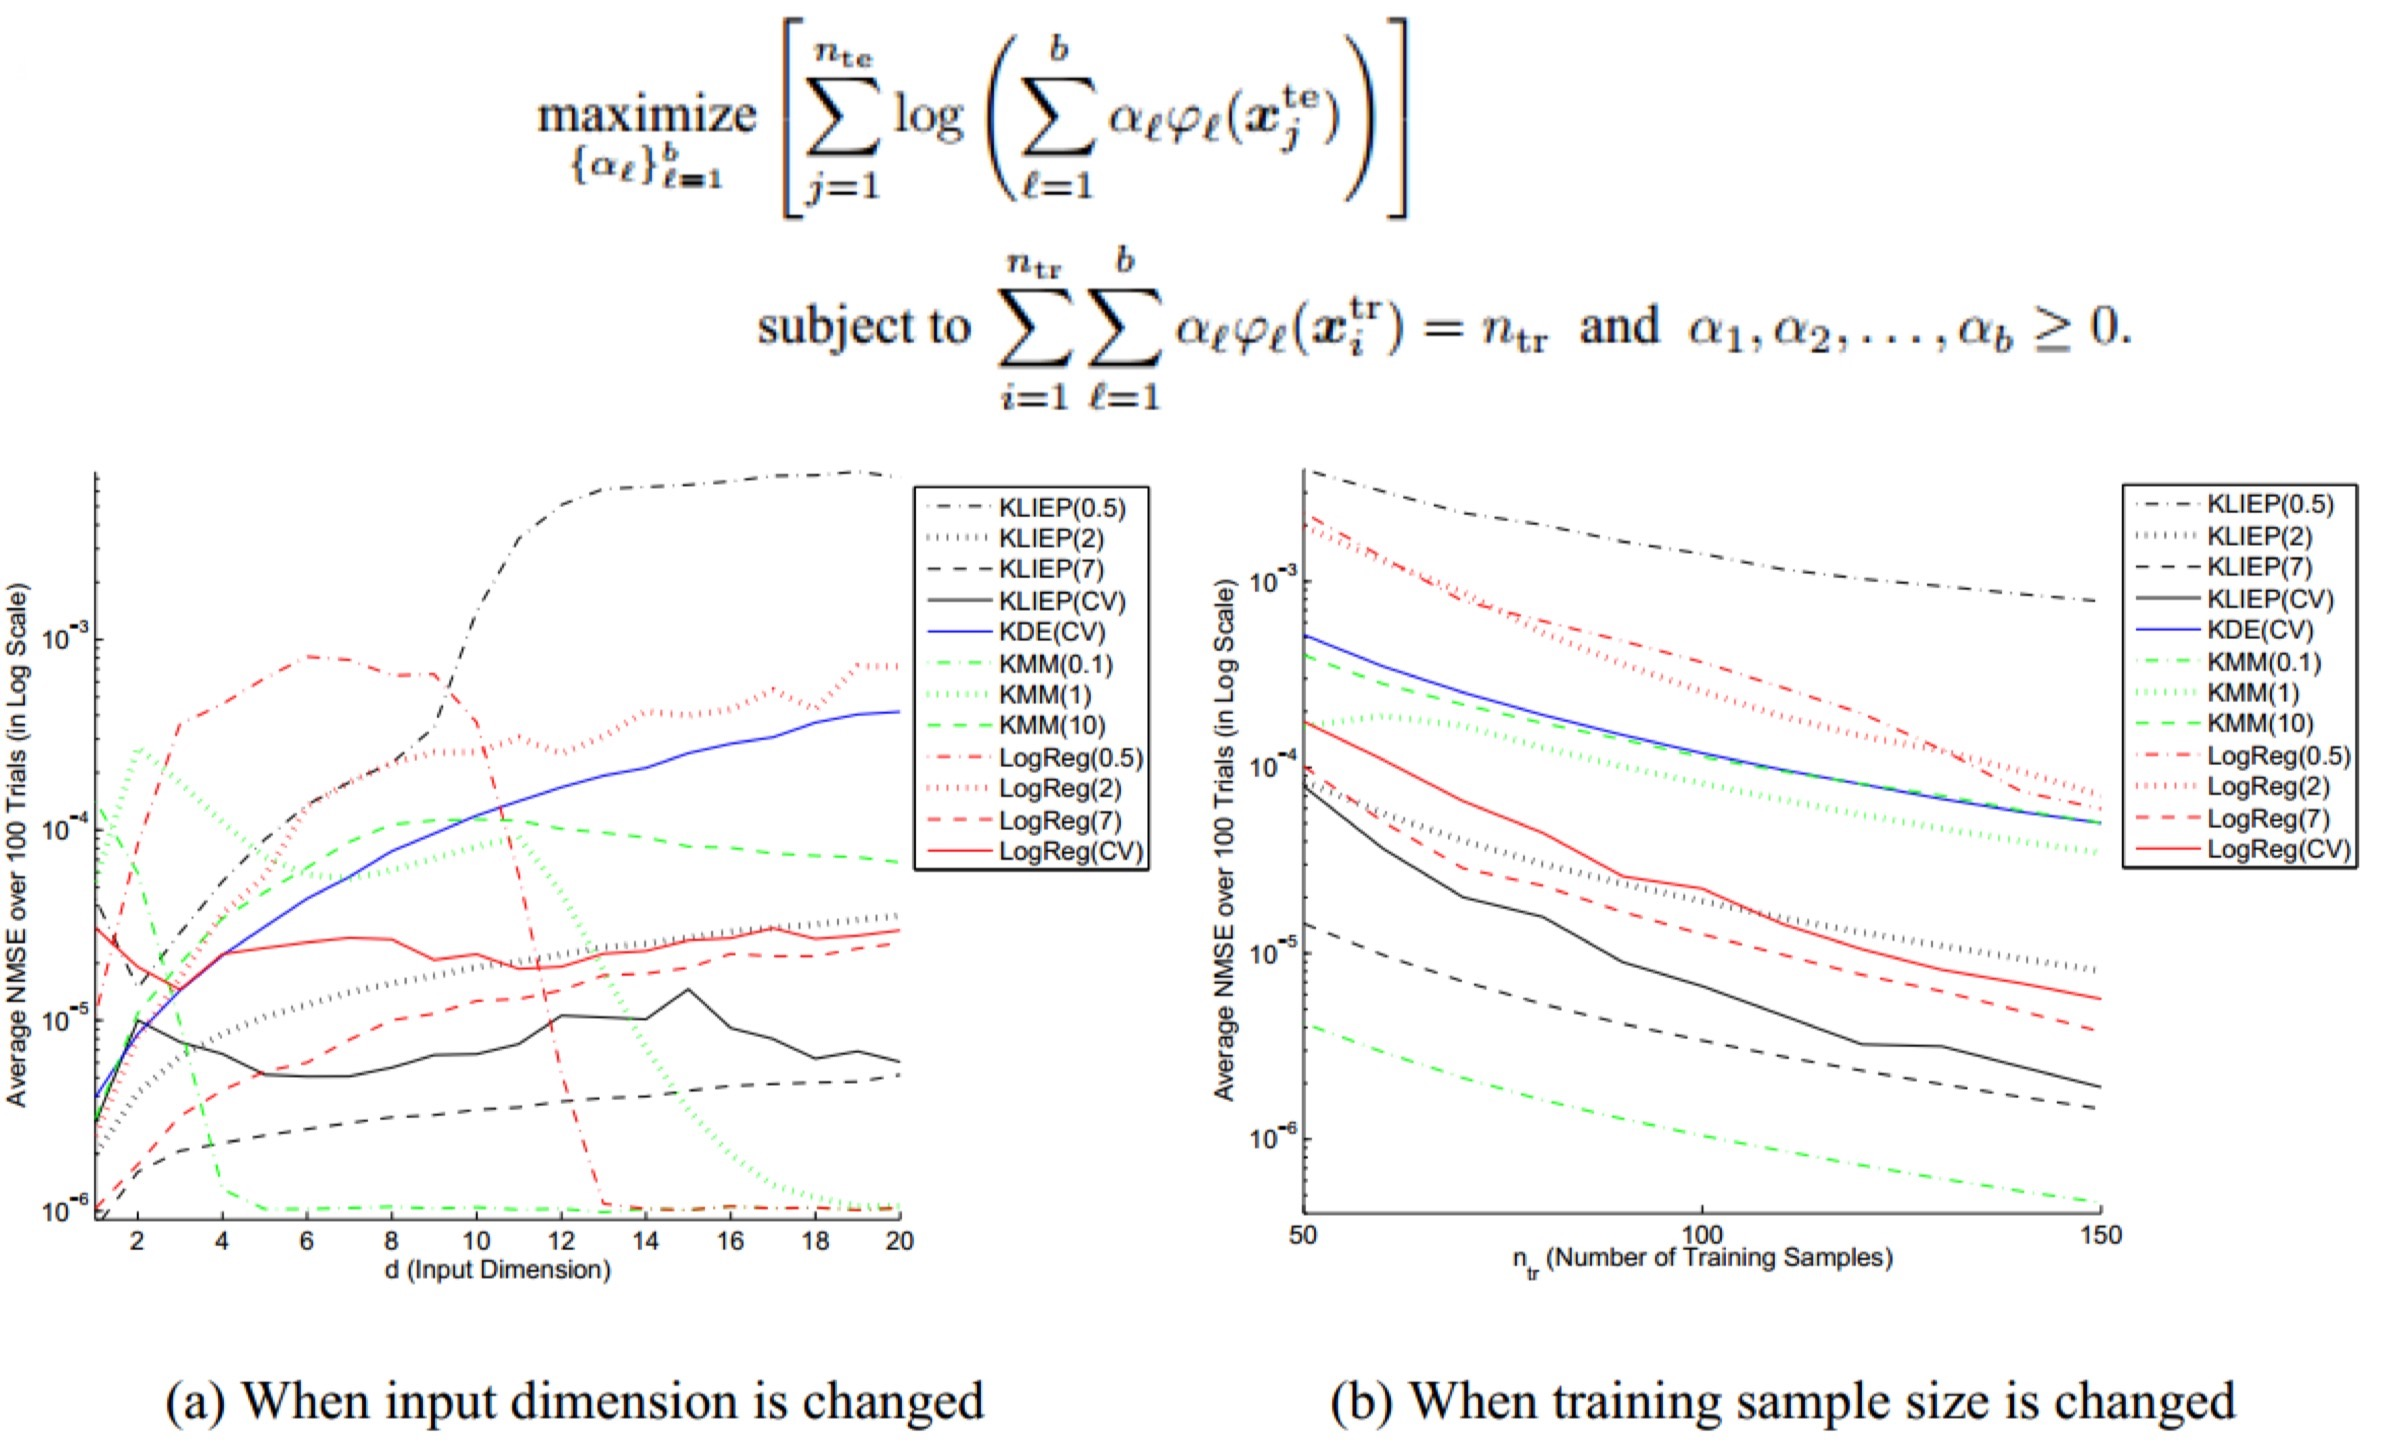
\includegraphics[width=0.7\textwidth]{csa.jpg}
    \end{figure}
\end{frame}

\begin{frame}
    \frametitle{迁移学习:域适配问题}
    \begin{itemize}
        \item 总结
        \begin{itemize}
            \item 通常假设源域和目标域的数据有着相同的条件分布,或者在高维空间里,有着相同的条件分布
            \item 这个假设是有一定局限性的,无法衡量源域和目标域之间相 似性,可能发生负迁移
        \end{itemize}
    \end{itemize}
\end{frame}
%%\subsection{深度迁移学习 (deep TL)}

\begin{frame}
    \frametitle{迁移学习:深度迁移学习}
    \begin{itemize}
        \item 利用深度神经网络的结构进行迁移学习
            \begin{itemize}
                \item 多层次的特征学习
            \end{itemize}
        \item 代表方法
            \begin{itemize}
                \item Joint CNN [Tzeng, ICCV-15]
                \item SHL-MDNN [Huang, ICASSP-13]
                \item Deep Adaptation Network (DAN) [Long, ICML-15]
                \item Domain Adversarial Training (DANN) [Ganin, ICML-15]
                \item Domain Separation Network (DSN) [Bousmalis, NIPS-16]
                \item Selective Adversarial Network (SAN) [Cao, CVPR-18]
            \end{itemize}
    \end{itemize}
\end{frame}

\begin{frame}
    \frametitle{迁移学习:深度迁移学习}
    \begin{itemize}
        \item 深度学习模型的迁移:定量分析
            \begin{itemize}
                \item unsupervised domain adaption Amazon‑>Webcam over time
            \end{itemize}
    \end{itemize}
    \begin{figure}
        \includegraphics[width=0.9\textwidth]{deep1.png}
    \end{figure}
\end{frame}

\begin{frame}
    \frametitle{迁移学习:深度迁移学习}
    \begin{itemize}
        \item Transferability of Layer‑wise Features \footfullcite{yosinski2014transferable}
    \end{itemize}
    \begin{figure}
        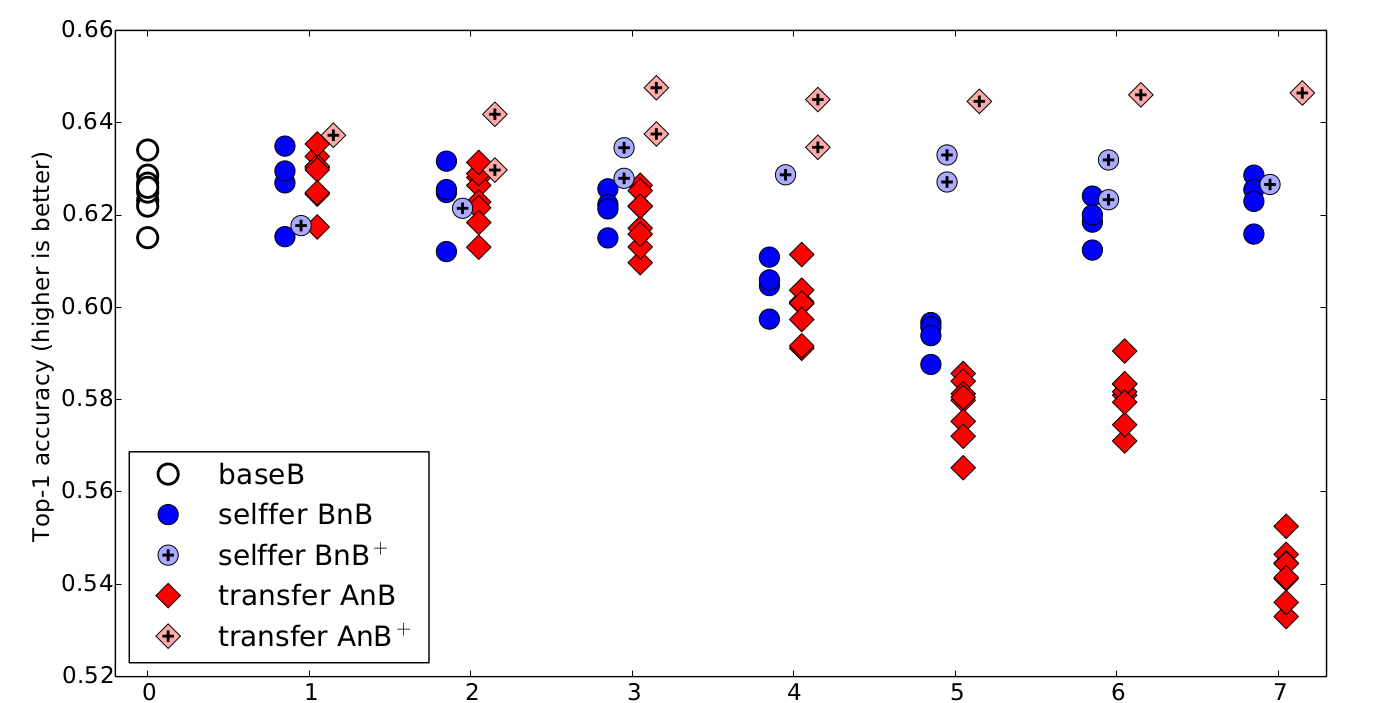
\includegraphics[width=0.8\textwidth]{transferable.png}
    \end{figure}
\end{frame}

\begin{frame}
    \frametitle{迁移学习:深度迁移学习}
    \begin{itemize}
        \item joint CNN [Tzeng, ICCV-15]
            \begin{itemize}
                \item 针对有稀疏标记的目标域数据,用CNN同时优化域之间的距离和迁移学习任务的损失
            \end{itemize}
    \end{itemize}
    \begin{figure}
        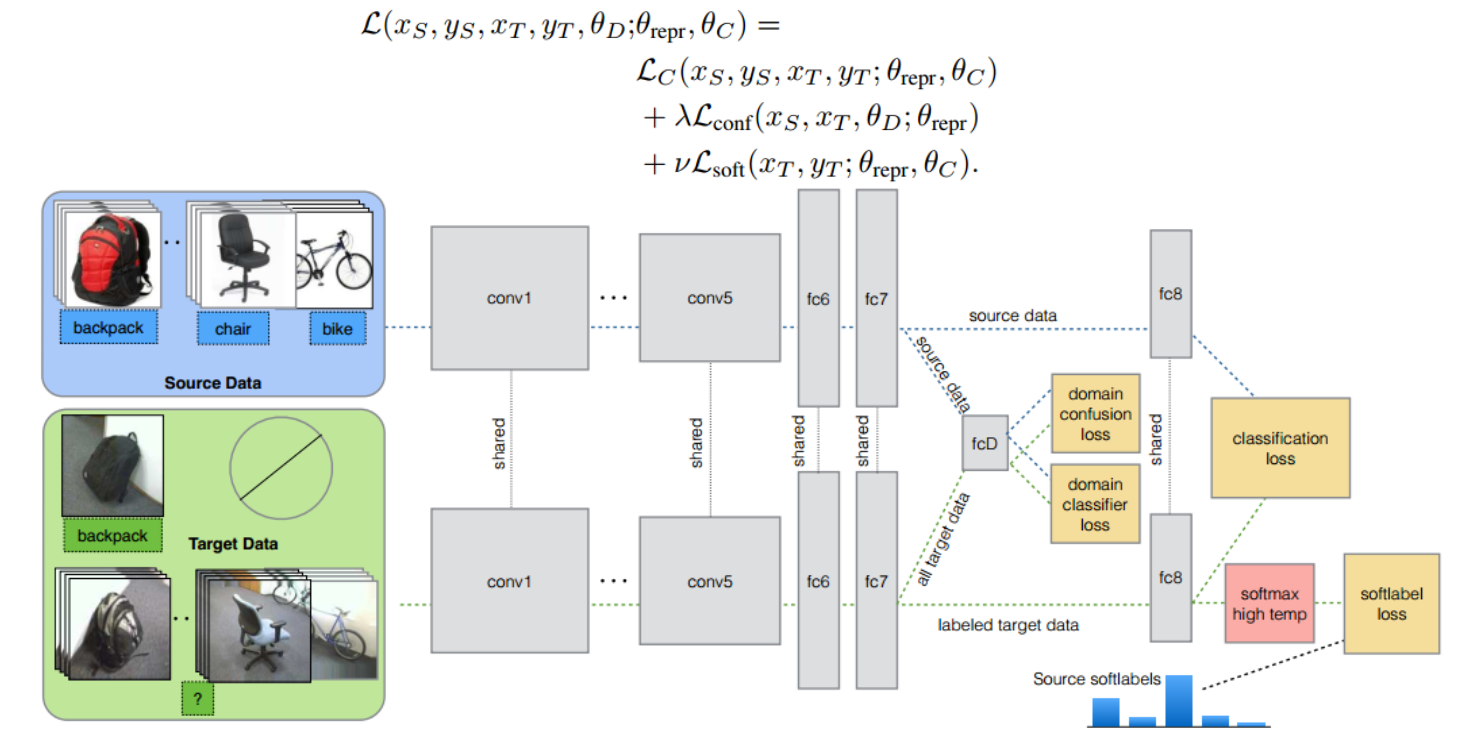
\includegraphics[width=0.9\textwidth]{jcnn.png}
    \end{figure}
\end{frame}

\begin{frame}
    \frametitle{迁移学习:深度迁移学习}
    \begin{itemize}
        \item SHL-MDNN [Huang, ICASSP-13]
            \begin{itemize}
                \item 在不同的学习网络之间共享隐藏层,通过不同的softmax层控制学习任务的不同
            \end{itemize}
    \end{itemize}
    \begin{figure}
        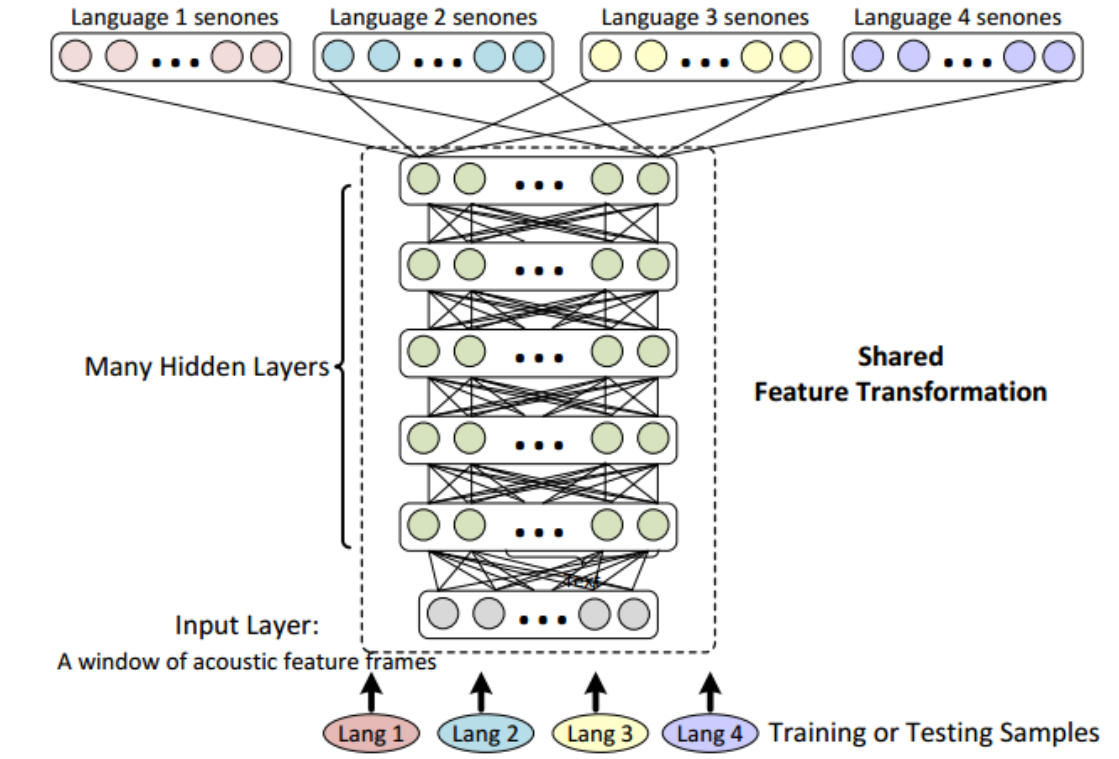
\includegraphics[width=0.7\textwidth]{shl-mdnn.png}
    \end{figure}
\end{frame}

\begin{frame}
    \frametitle{迁移学习:深度迁移学习}
    \begin{itemize}
        \item Deep Adaptation Network (DAN)
    \end{itemize}
    \begin{figure}
        \includegraphics[width=0.8\textwidth]{dan.png}
    \end{figure}
\end{frame}

\begin{frame}
    \frametitle{迁移学习:深度迁移学习}
    \begin{itemize}
        \item Domain Adversarial Training (DANN) [Ganin, ICML-15]
    \end{itemize}
    \begin{figure}
        \includegraphics[width=0.9\textwidth]{dann.png}
    \end{figure}
\end{frame}

\begin{frame}
    \frametitle{迁移学习:深度迁移学习}
    \begin{itemize}
        \item Domain Separation Network (DSN) [Bousmalis, NIPS-16]
    \end{itemize}
    \begin{figure}
        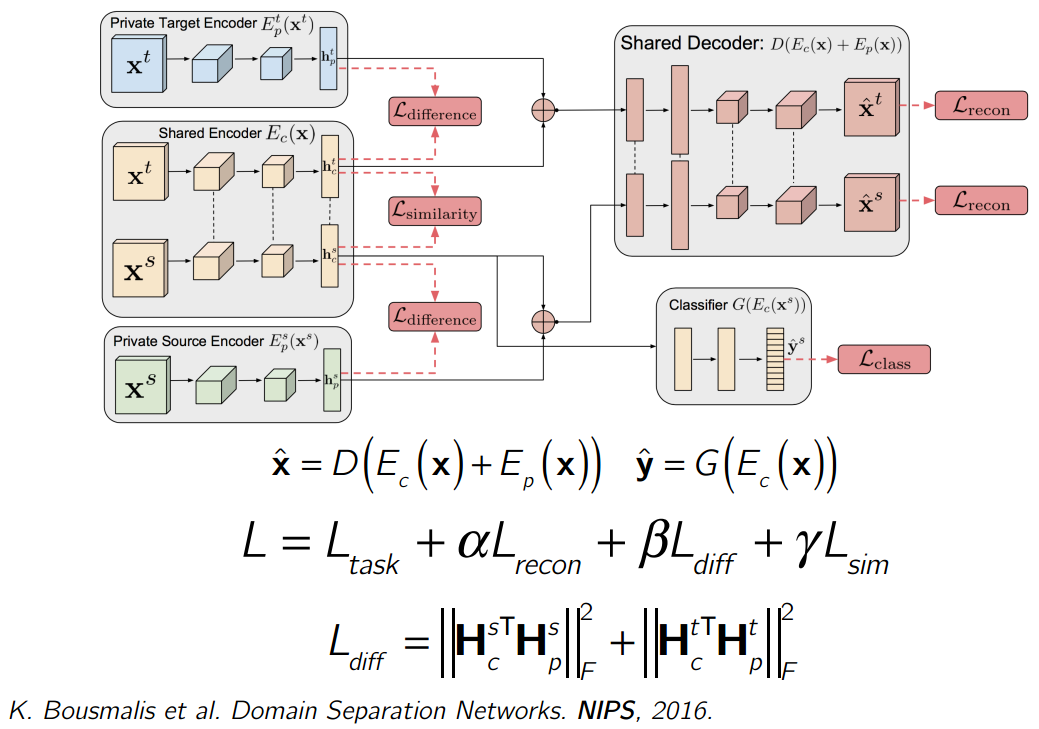
\includegraphics[width=0.8\textwidth]{dsn.png}
    \end{figure}
\end{frame}

\begin{frame}
    \frametitle{迁移学习:深度迁移学习}
    \begin{itemize}
        \item Selective Adversarial Network (SAN) [Cao, CVPR-18]
            \begin{itemize}
                \item Partial Transfer Learning
                \item 源域的标签包含目标域的标签
            \end{itemize}
    \end{itemize}
    \begin{figure}
        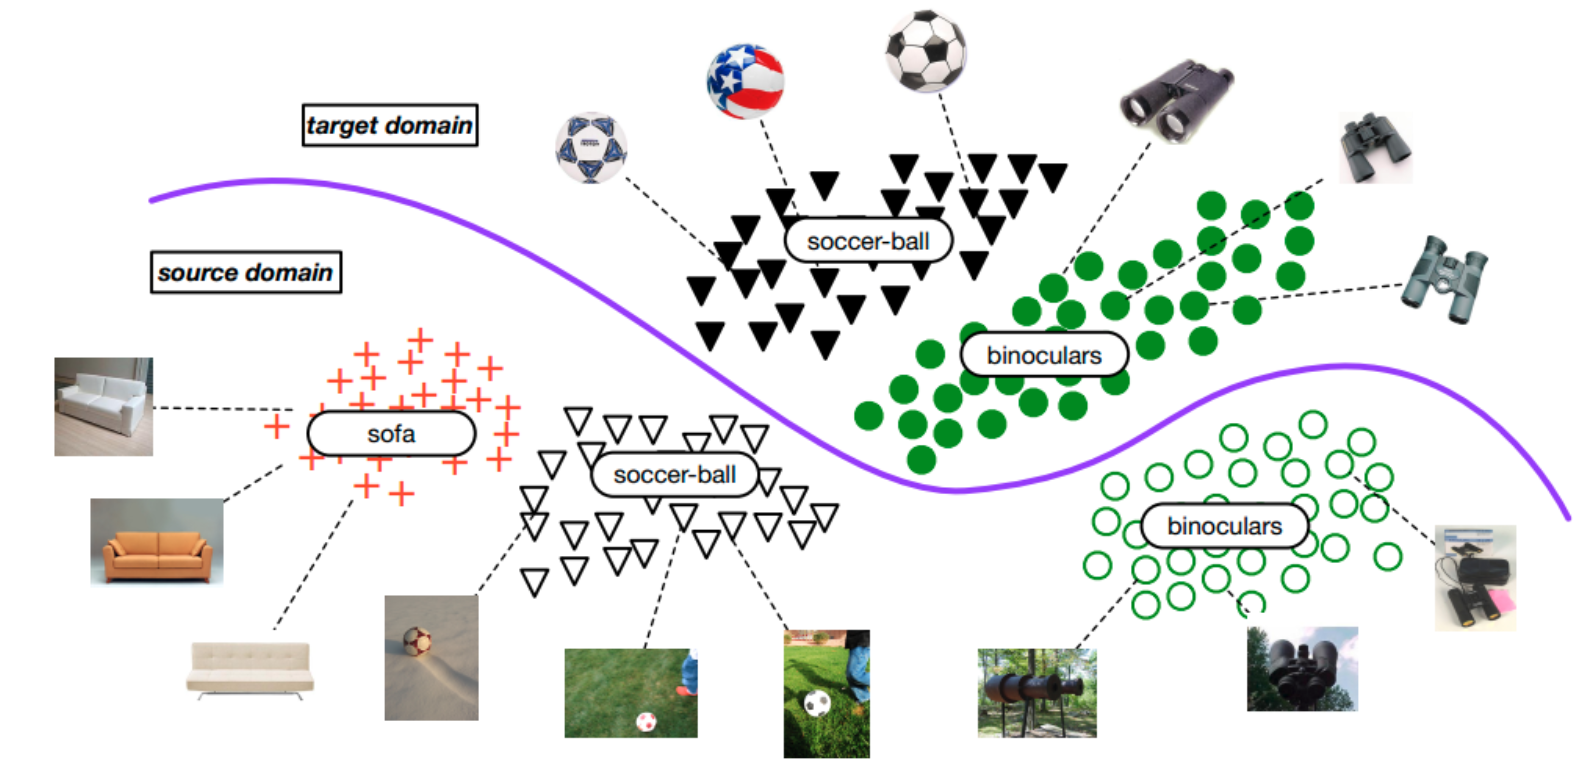
\includegraphics[width=0.8\textwidth]{san1.png}
    \end{figure}
\end{frame}

\begin{frame}
    \frametitle{迁移学习:深度迁移学习}
    \begin{itemize}
        \item Selective Adversarial Network (SAN) [Cao, CVPR-18]
    \end{itemize}
    \begin{figure}
        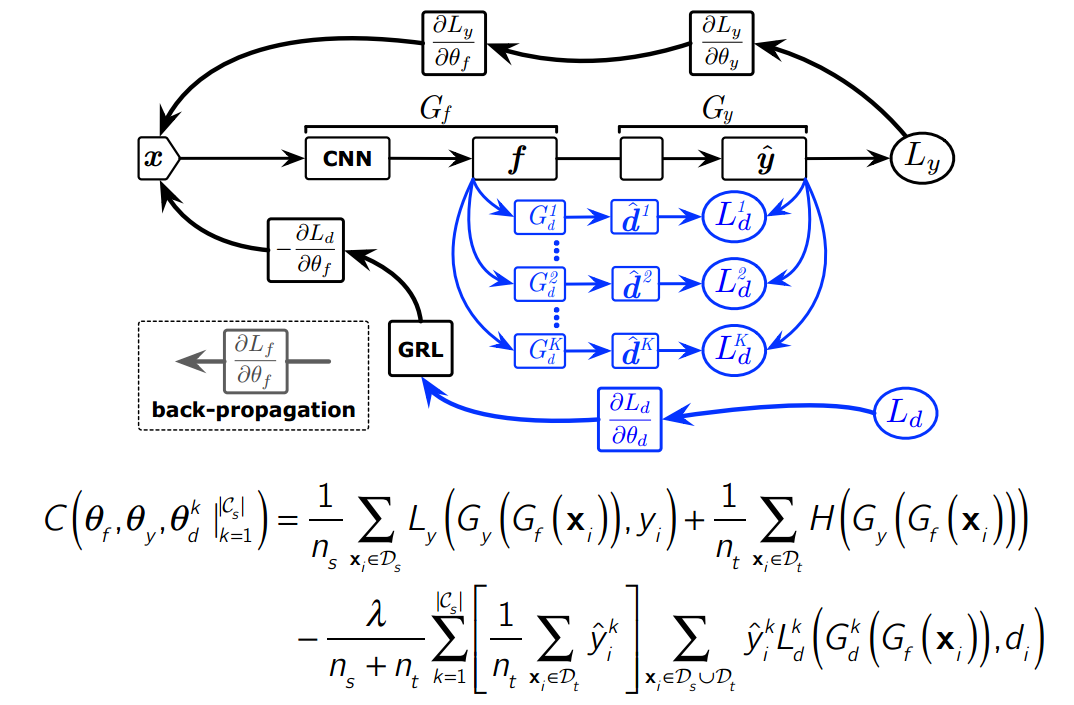
\includegraphics[width=0.8\textwidth]{san2.png}
    \end{figure}
\end{frame}

\begin{frame}
    \frametitle{迁移学习:深度迁移学习}
    \begin{itemize}
        \item 总结
        \begin{itemize}
            \item 迁移学习大增强了模型的泛化能力
            \item 深度学习可以深度表征域中的知识结构
            \item 深度学习+迁移学习还可大有作为
        \end{itemize}
    \end{itemize}
\end{frame}
%%\subsection{多源迁移学习 (multi-source TL)}

\begin{frame}
    \frametitle{迁移学习:多源迁移学习}
    \begin{itemize}
        \item 多源迁移学习
            \begin{itemize}
                \item 问题定义:多个源域和目标域,如何进行有效的域筛选,从而进行迁移?
            \end{itemize}
        \item 代表方法
            \begin{itemize}
                \item TrAdaBoost [Dai, ICML-07]
                \item MsTL-MvAdaboost [Xu, ICONIP-12]
                \item Consensus regularization [Luo, CIKM-08]
                \item Transitive transfer learning [Tan, KDD-15]
                \item Distant domain TL [Tan, AAAI-17]
            \end{itemize}
    \end{itemize}
\end{frame}

\begin{frame}
    \frametitle{迁移学习:多源迁移学习}
    \begin{itemize}
        \item TrAdaBoost [Dai, ICML-07]
            \begin{itemize}
                \item 利用Boost的技术过滤掉多个源域中与目标域不相似的样本,然后进行实例迁移学习
            \end{itemize}
    \end{itemize}
    \begin{figure}
        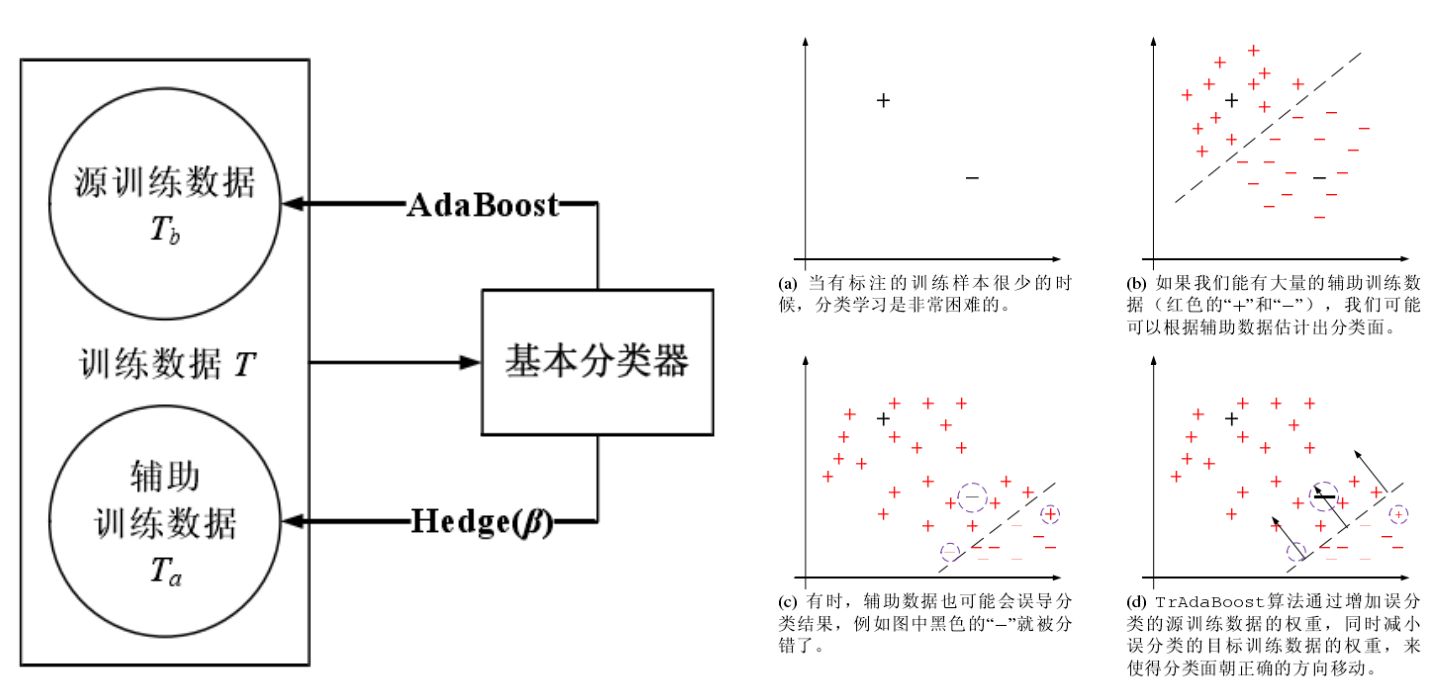
\includegraphics[width=0.9\textwidth]{tradaboost.png}
    \end{figure}
\end{frame}

\begin{frame}
    \frametitle{迁移学习:多源迁移学习}
    \begin{itemize}
        \item MsTL-MvAdaboost [Xu, ICONIP-12]
            \begin{itemize}
                \item 不仅考虑源域和目标域的样本相似度情况,同时以多视图学习的目标来进行统一的迁移
            \end{itemize}
        \item Consensus regularization [Luo, CIKM-08]
            \begin{itemize}
                \item 同时在源域和伪标注的目标域上训练分类器,利用一致性约束进行知识的迁移
            \end{itemize}
    \end{itemize}
\end{frame}

\begin{frame}
    \frametitle{迁移学习:多源迁移学习}
    \begin{itemize}
        \item Transitive transfer learning [Tan, KDD-15]
            \begin{itemize}
                \item 在两个相似度不高的域中,利用从第三方中学习到的相似度
                关系,完成知识的传递迁移
            \end{itemize}
    \end{itemize}
    \begin{figure}
        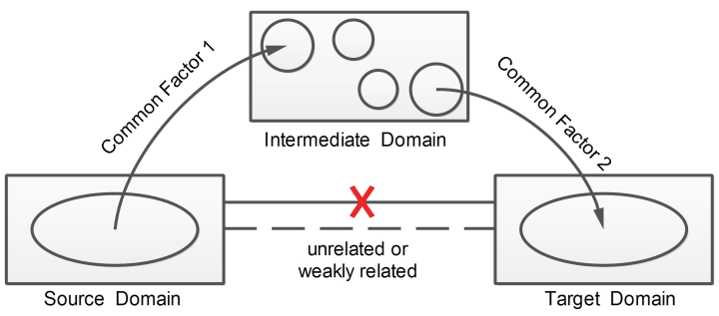
\includegraphics[width=0.9\textwidth]{ttl.jpg}
    \end{figure}
\end{frame}

\begin{frame}
    \frametitle{迁移学习:多源迁移学习}
    \begin{itemize}
        \item Distant domain TL [Tan, AAAI-17]
            \begin{itemize}
                \item 在相似度极低的两个域进行迁移时,用autoencoder自动从
                多个中间辅助域中选择知识,完成迁移
            \end{itemize}
    \end{itemize}
    \begin{figure}
        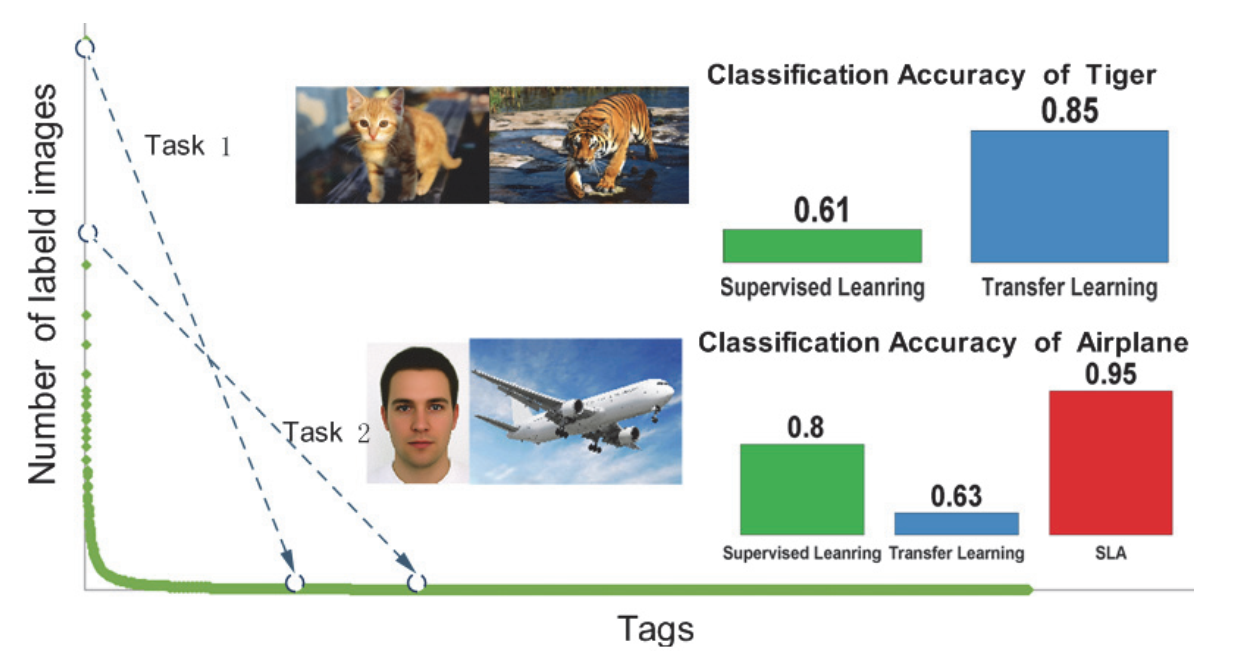
\includegraphics[width=0.9\textwidth]{sla.png}
    \end{figure}
\end{frame}

\begin{frame}
    \frametitle{迁移学习:多源迁移学习}
    \begin{itemize}
        \item 总结
        \begin{itemize}
            \item 多源迁移学习可以有效利用存在的多个可用域,综合起来进
            行迁移,达到较好的效果
            \item 如何衡量多个域之间的相关性还是一个问题
            \item 对多个域的利用方法也存在一定挑战性
        \end{itemize}
    \end{itemize}
\end{frame}
%%%%%%%%%%%%%%%%%%
\section{总结}

\begin{frame}
    \frametitle{19年下半年计划}
    \begin{itemize}
        \item 将IJCAI的内容扩展到TKDE上,目前文章已经写完了,仍需要补充实验(ensemble learning, 其余的多视图聚类方法)
        \item 一些新的idea
            \begin{itemize}
                \item 扩展:系数约束是 $\ell_{2}$的(我们并不想要稀疏的解),而将约束调整为 $\ell_{1}$后,可以考虑增加diversity-induced的惩罚项。
                \item 核矩阵之间的相似度度量:hilbert-schmidt independence criterion(HSIC)
            \end{itemize}

    \end{itemize}
\end{frame}

\begin{frame}
    \frametitle{ICCV审稿} 
    \begin{figure}
        \includegraphics[width=0.8\textwidth]{figures/iccv1.png} 
    \end{figure}          
\end{frame}

\begin{frame}
    \frametitle{ICCV审稿} 
    \begin{figure}
        \includegraphics[width=0.8\textwidth]{figures/iccv2.png} 
    \end{figure}          
\end{frame}

\begin{frame}
    \frametitle{19年下半年计划}
    \begin{itemize}
        \item 谢谢大家
    \end{itemize}
\end{frame}

\end{document}